\documentclass{article}
\usepackage{amssymb,amsthm,amsmath}
\usepackage{fullpage}
\usepackage{url}
\usepackage{comment}
\usepackage{tikz}
\usepackage{tikz-cd}
\usepackage{listings}
\usepackage{multicol}
\usepackage{amsmath}
\usepackage{stmaryrd}
\usetikzlibrary{quotes}
\tikzset{>=latex}

%%%%%%%%%%%%%%%%%%%%%%%%%%%%%%%%%%%%%%%%%%%%%%%%%%%%%%%%%%%%%%%%%
%% Macros

\newcommand{\nboxtimes}[2]{\,\,~{^{#1}\boxtimes^{#2}}~\,\,}
\newcommand{\mm}{\texttt{\textminus}}
\newcommand{\pp}{\texttt{+}}
\newcommand{\inl}[1]{\textsf{inl}~#1}
\newcommand{\inr}[1]{\textsf{inr}~#1}
\newcommand{\idv}[3]{#2 \xrightarrow{#1} #3}
\newcommand{\cp}[3]{#1\stackrel{#2}{\bullet}#3}
\newcommand{\idt}[3]{#2 \equiv_{#1} #3}
\newcommand{\idrt}[3]{#3 \equiv_{#1} #2}
\newcommand{\refl}[1]{\textsf{refl}~#1}
%% \newcommand{\lid}{\textsf{lid}}
\newcommand{\alt}{~|~}
%% \newcommand{\rid}{\textsf{rid}}
\newcommand{\linv}{l!}
\newcommand{\rinv}{r!}
\newcommand{\invinv}{!!}
\newcommand{\assoc}{\circ}
\newcommand{\identlp}{\mathit{unite}_+\mathit{l}}
\newcommand{\identrp}{\mathit{uniti}_+\mathit{l}}
\newcommand{\identlsp}{\mathit{unite}_+\mathit{r}}
\newcommand{\identrsp}{\mathit{uniti}_+\mathit{r}}
\newcommand{\swapp}{\mathit{swap}_+}
\newcommand{\assoclp}{\mathit{assocl}_+}
\newcommand{\assocrp}{\mathit{assocr}_+}
\newcommand{\identlt}{\mathit{unite}_*\mathit{l}}
\newcommand{\identrt}{\mathit{uniti}_*\mathit{l}}
\newcommand{\identlst}{\mathit{unite}_*\mathit{r}}
\newcommand{\identrst}{\mathit{uniti}_*\mathit{r}}
\newcommand{\swapt}{\mathit{swap}_*}
\newcommand{\assoclt}{\mathit{assocl}_*}
\newcommand{\assocrt}{\mathit{assocr}_*}
\newcommand{\absorbr}{\mathit{absorbr}}
\newcommand{\absorbl}{\mathit{absorbl}}
\newcommand{\factorzr}{\mathit{factorzr}}
\newcommand{\factorzl}{\mathit{factorzl}}
\newcommand{\dist}{\mathit{dist}}
\newcommand{\factor}{\mathit{factor}}
\newcommand{\distl}{\mathit{distl}}
\newcommand{\factorl}{\mathit{factorl}}
\newcommand{\distz}{\mathit{absorbr}}
\newcommand{\iso}{\leftrightarrow}
\newcommand{\proves}{\vdash}
\newcommand{\idc}{\mathit{id}\!\!\leftrightarrow}
\newcommand{\Rule}[4]{
\makebox{{\rm #1}
$\displaystyle
\frac{\begin{array}{l}#2 \\\end{array}}
{\begin{array}{l}#3      \\\end{array}}$
 #4}}
\newcommand{\jdg}[3]{#2 \proves_{#1} #3}


\title{Embracing the Laws of Physics: \\ Three Reversible Models of Computation}
\author{Jacques Carette \qquad\qquad Roshan P. James \qquad\qquad Amr Sabry \\
McMaster University \qquad\qquad Google \qquad\qquad Indiana University}

\newtheorem{thm}{Theorem}[section]
\newtheorem{defn}{Definition}[section]
\newtheorem{prop}{Proposition}[section]

\newcommand{\amr}[1]{\fbox{Amr says:} \textbf{#1}}
\newcommand{\jc}[1]{\fbox{Jacques says:} \textbf{#1}}
\newcommand{\roshan}[1]{\fbox{Roshan says:} \textbf{#1}}

\newcommand{\lcal}{\ensuremath{\lambda}-calculus}

\newcommand{\fin}[1]{\ensuremath{\left[#1\right]}}
\newcommand{\Nat}{\ensuremath{\mathbb{N}}}
\newcommand{\true}{\mathit{true}}
\newcommand{\false}{\mathit{false}}


\newcommand{\kw}[1]{{\scriptsize{\textbf{\texttt{#1}}}}}
\newcommand{\ctr}[1]{{\scriptsize{\texttt{#1}}}}
\newcommand{\inline}[3]{\ctr{#1} \textasciitilde \ctr{#2}:\ctr{#3}}

\begin{document}
\maketitle 

\begin{abstract}
  Our main models of computation (the Turing Machine and the RAM) and
  most modern computer architectures make fundamental assumptions
  about which primitive operations are realizable on a physical
  computing device. The consensus is that these primitive operations
  include logical operations like conjunction, disjunction and
  negation, as well as reading and writing to a (large) collection to
  memory locations. This perspective conforms to a macro-level view of
  physics and indeed these operations are realizable using macro-level
  devices involving thousands of electrons. This point of view is
  however incompatible with computation realized using quantum devices
  or analyzed using elementary thermodynamics as both these
  fundamental physical theories imply that information is a conserved
  quantity of physical processes and hence of primitive computational
  operations.

  Our aim is re-develop foundational computational models in a way
  that embraces the principle of conservation of information. We first
  define what information is and what its conservation means in a
  computational setting. We emphasize the idea that computations,
  whatever they are, must be reversible transformations on
  data. Thinking topologically, one can think of data as modeled using
  topological spaces and programs as modeled by reversible
  deformations of these spaces. We then illustrate this idea using
  three notions of data and their associated reversible computational
  models. The first instance only assumes unstructured finite data,
  i.e., discrete topological spaces. The corresponding notion of
  reversible computation is that of permutations. We show how this
  simple model subsumes conventional computations on finite sets. We
  then consider a modern structured notion of data based on the
  Curry-Howard correspondence between logic and type theory. We
  develop the corresponding notion of reversible deformations using a
  sound and complete programming language for witnessing type
  isomorphisms and proof terms for commutative semirings.  We then
  ``move up a level'' to examine spaces that treat programs as data
  which is a crucial notion for any universal model of computation. To
  derive the corresponding notion of reversible programs between
  programs, i.e., reversible program equivalences, we look at the
  ``higher dimensional'' analog to commutative semirings: symmetric
  rig groupoids. The coherence laws for these groupoids turn out to be
  exactly the sound and complete reversible program equivalences we
  seek.
 
  We conclude with some possible generalizations inspired by homotopy
  type theory and survey several open directions for further research.

%%  Something about Theseus?
\end{abstract}

% * Reversibility intro / motivation as we  have now more or less

% * Thesis statement: programs are reversible deformations on data /
%    spaces, almost necessarily by definition

% * Focus now is on data

% * If data is plain finite sets, programs become permutations (deformations on finite sets).

% * If data is structured trees, we get Pi.

% * Explain Pi with examples.

% * If data is itself deformations-on-finite-sets, then the
%   deformations between them become something quite
%   interesting. Explain Pi level 2 with examples.

% * Conclude with thoughts regarding other kinds of data that can be
%   plugged in into that story.

%%%%%%%%%%%%%%%%%%%%%%%%%%%%%%%%%%%%%%%%%%%%%%%%%%%%%%%%%%%%%%%%%
\section{Reversibility, the Missing Principle}

What kind of operations can computers perform? This question was
answered several times in the last hundred years, where each answer
proposes an abstract \emph{model of computation} that specifies
allowable operations and (usually) their cost. The emerging consensus,
reflected in both early models of computations such as the Turing
Machine and the RAM as well as in the early Von Neumann and in modern
computer architectures, is that basic computer operations include
logical operations like conjunction, disjunction, and negation, as
well as reading from and writing to a large (infinite) collection of
memory locations. From this small set of primitive operations emerges
all higher-level programming languages and abstractions.

No doubt, this consensus on the available primitive physical
operations has been successful. And no doubt, these operations
\emph{can} indeed be performed on a computer. Yet, today, with a
possible quantum computing revolution in sight and with unprecedented
explosion in embedded computers and cyber-physical systems, there are
reasons to re-think this foundational question again. In fact, the
calls to re-think this foundational question have been proclaimed by
physicists more than forty years ago as the following two quotes
testify:

\begin{quote}
  \textbf{Toffoli 1980~\cite{toffoli:1980}:} Mathematical models of
  computation are abstract constructions, by their nature unfettered
  by physical laws. However, if these models are to give indications
  that are relevant to concrete computing, they must somehow capture,
  albeit in a selective and stylized way, certain general physical
  restrictions to which all concrete computing processes are
  subjected.

  \textbf{Feynman 1982~\cite{springerlink:10.1007/bf02650179}:}
  Another thing that has been suggested early was that natural laws
  are reversible, but that computer rules are not. But this turned out
  to be false; the computer rules can be reversible, and it has been a
  very, very useful thing to notice and to discover that. This is a
  place where the relationship of physics and computation has turned
  itself the other way and told us something about the possibilities
  of computation. So this is an interesting subject because it tells
  us something about computer rules.
\end{quote}

\noindent These quotes by Toffoli and Feynman both highlight the
consequences of two obvious observations: (i) all the operations that
a computer performs reduce to basic physical operations; and (ii)
there is a mismatch between the logical operations of a typical model
of computation (which are logically irreversible) and the fundamental
laws of physics (which are reversible). One could certainly dismiss
the mismatch as irrelevant to the practice of computing but our thesis
is that the next computing revolution is likely to be founded on
revised models of computation that are designed to in closer harmony
with the laws of physics.

After a detailed introduction on the origins of ``logically
reversibile computer operations'' and an excursion into the origins of
``irreversible computer operations'', we will develop in detail three
reversible models of computation and discuss their potential
applications.

%%%%%%%%%
\paragraph*{Maxwell's Demon.}
To fully appreciate the missing principle of ``reversibility'' in
conventional computing, we go back to an old thought experiment by
J. C. Maxwell. The details are codified in a letter that Maxwell wrote
to P. G Tait in 1867 -- the letter, whose ideas are now known as
\emph{Maxwell's Demon}, tells of a thought experiment that seems to
indicate that intelligent beings can somehow violate the second law of
thermodynamics, thereby violating physics itself. Many resolutions
were offered for this conundrum (for a compilation, see the book by
Leff and Rex~\cite{leff1990}), but none withstood careful scrutiny
until the establishment of \emph{Landauer's Principle} in
1961~\cite{Landauer:1961} -- a principle whose experimental validation
happened recently in 2012~\cite{berut2012experimental}.

Maxwell's demon appears to violate the second law of thermodynamics by
having a tiny ``intelligence'' observing the movement of individual
particles of a gas and separating fast moving particles from slow
moving ones, thereby reducing the total entropy of the
system. Landauer's resolution of the demon relied on two ideas that
took root only a few decades earlier: the formal notion of computation
(through the work of Turing and Church, 1936) and the formal notion of
information (through the work of Shannon, 1948). Landauer reasoned
that the computation done by the finite brain of the demon, involves
getting information about the movement of molecules, storing that
information, analyzing that information to act on it, and then --- and
this is the critical step --- overwriting it to make room for the next
computation.  In other words, the computation that is manipulating
information in the demon's brain \textit{must be thermodynamic work},
thereby bringing the demon back into the fold of physics.

This is a strange and wonderful idea: information, physics, and
computation are inextricably linked. In contrast, when the early
models of computation were developed, there was no compelling reason
to the take the information content of computations into consideration
-- in fact, at that time there was no quantifiable notion of
information. These models followed in the footsteps of logic where,
following hundreds of years of tradition, the truth of a statement was
seen as ``absolute'' and independent of any reasoning, understanding,
or action. Statements were either true or false with no regard to any
``observer'' and the idea that statements had information content that
should be preserved was outside the classical understanding of
logic. Hence the fact that conventional logic operations such as
conjunction and disjunction were logically irreversible and hence lose
information was not a concern. Landauer's observation implied however
that ideas in each field have consequences for the
other~\cite{bennett:1973:lrc,bennett1985fundamental,bennett2010notes,bennett2003notes,baker:1992:nft,baez2011physics,dblp:conf/csfw/malacarias12}. To
really appreciate this fact, we delve deeper into the origin of our
computational models and argue that they are essentially reflections
of contemporary laws of physics.

%%%%%%%%%
\paragraph*{Origins of Computational Models.}
Current high-level programming languages as well as current hardware
are both based on Boolean Logic -- which really ought to be called
\emph{Piercean logic}, as Boole had a rather different conception of
logic which is rather far from our current models.  Nevertheless,
going back to Boole's 1853 book entitled \emph{An Investigation of the
  Laws of Thought, on which are Founded the Mathematical Theories of
  Logic and Probabilities}, we find that the opening sentence of Ch.~1 is:
\begin{quote}
  The design of the following treatise is to investigate the fundamental laws
  of those operations of the mind by which reasoning is performed; \ldots
\end{quote}
which clearly identifies the ``source'' of the logical laws as
mirroring Boole's understanding of human reasoning. A few chapters
later, we find:
\begin{quote}
  \textbf{Proposition IV.}  That axiom of metaphysicians which is termed the
  principle of contradiction, and which affirms that it is impossible for any
  being to possess a quality, and at the same time not to possess it, is a
  consequence of the fundamental law of thought, whose expression is $x^2 =
  x$.
\end{quote}
This ``law'' is reasonable in a classical world but is violated by the
postulates of quantum mechanics. Although a detailed historical
analysis of Boole's ideas in the light of modern physics is beyond our
scope, the above quotes should convey the idea that our elementary
computing notions date back to ideas that were thought reasonable in
the late 1800s. 

Machines that ``compute'' are quite old. M\"{u}ller (1786) first
conceived of the idea of a ``difference machine'', which Babbage
(1819--1822) was able to construct. There are other computer
precursors as well -- the first stored programs were actually for
looms, most notably those of Bouchon (1725) which operated on a paper
tape, and Jacquard (1804) which operated by chains of punched cards.
But it was only in the 20th century that computer science emerged as a
formal discipline. One of the pioneering works was Alan Turing's
seminal paper in 1936 which established the idea that computation has
a formal interpretation and that all computability can be captured
within a formal system. Implicit in this achievement however is the
idea that abstract models of computation are just that --
\emph{abstractions of computation realized in the physical world.}
Indeed, going back to Turing's 1936 article \emph{On Computable
  Numbers, with an Application to the Entscheidungsproblem,}, the
opening sentence of Sec. 1 is:
\begin{quote}
  We have said that the computable numbers are those whose decimals are
  calculable by finite means \ldots the justification lies in the fact that
  the human memory is necessarily limited.
\end{quote}
In Sec. 9, we find:
\begin{quote}
  I think it is reasonable to suppose that they can only be squares
  whose distance from the closest of the immediately previously
  observed squares does not exceed a certain fixed amount.
\end{quote}
It is worth noting that these assumptions are both physical (on
distances) and metaphysical (on restrictions of the mind).  If we take
the human mind to be a physical ``machine'' which does computation,
then when both of the above assumptions are translated to the language
of physics, they embody what is known as the ``Bekenstein bound'',
which is an upper limit on the amount of information that can be
contained within a given finite region of space. A detailed historical
account of these ideas in the context of modern physics is again
beyond our scope. However, the quotes above, like the ones before,
should convey the ideas that our theories of computation and
complexity are based on some physical assumptions that Turing and
others found reasonable in the 1930s.

To summarize, a major achievement of computer science has been the
development of abstract models of computation that shield the
discipline from rapid changes in the underlying technology. Yet, as
effective as these models have been, one must note that they
\emph{embody several implicit physical assumptions} and these
assumptions are based on a certain understanding of the laws of
physics. Our understanding of physics has evolved tremendously since
1900!  Thus it is time to revisit these abstractions, especially with
respect to quantum mechanics.  Indeed one should take the physical
principles underlying quantum mechanics, the most successful physical
theory known to us and adapt computation to ``learn'' from these
principles.  In the words of Girard:
\begin{quote}
  In other terms, what is so good in logic that quantum physics should
  obey?  Can't we imagine that our conceptions about logic are wrong,
  so wrong that they are unable to cope with the quantum miracle?
  [\ldots] Instead of teaching logic to nature, it is more reasonable
  to learn from her. Instead of interpreting quantum into logic, we
  shall interpret logic into quantum (Girard 2007).
\end{quote}

There are, in fact, many different quantum mechanical principles which
are at odds with our current models of computation. In this paper, we
will focus on the previously identified principle of
\emph{reversibility}. In more detail, we will view data as an explicit
representation of \emph{information} and programs as processes that
transform information in a reversible way, i.e., processes that are
subject to the physical principle of \emph{conservation of
  information.} We will formalize this idea and follow its
consequences, which will turn out to be far reaching.

%%%%%%%%%
\paragraph*{Programs as Reversible Deformations.}

To better understand the essence of ``conservation of information'' in
the context of computing, we first look for analogous ideas in
physics, but this time at the macro scale. Viewing information as a
physical object, what does it mean to transform an object in such a
way that we do not lose its fundamental character?

For rigid objects (like a chair), the only such transformations are
translations and rotations. But what about something more flexible,
with multiple representations, such as a water balloon?  Such objects
can be \emph{deformed} in various ways, but still retain their
fundamental character -- as long as we do not puncture them or
over-stretch them. Ignoring material characteristics
(i.e. over-stretching), what is special about these deformations, as
well as for translations and rotations, is that they correspond to
continuous maps, with a continuous inverse. In fact, even more is
true: they are analytic maps, with analytic inverses. For our purpose,
the most important part is that such maps are infinitely
differentiable.  In other words, not only is there an inverse to the
deformation, but its derivative is also invertible, and so on.

When we look around, we find many different words for related
concepts: isomorphism, equivalence, sameness, equality,
interchangeability, comparability, and correspondence, to name a
few. Some of these are informal concepts, while others have formal
mathematical meaning.  More importantly, even amongst the formal
concepts, there are differences -- which is why there are so many of
them! Because there are many such notions, we also need to walk our
way through them to find the one which is ``just right''. Thus we seek
a concept which is neither too strong nor too weak, that will express
when some structured information should be treated as ``the same''.
We can draw an analogy with topology: in topology, all point sets can
always be equipped with either the discrete or the indiscrete
topology, but both of these extremes are rarely useful. We will
develop our working notion of ``sameness'' as we go through the
various components that make up a programming language.

Starting from the physical perspective, whatever our notion of data
is, we will be interested in programs as representing transformations
of that data which are reversible. In other words, we want our
programs-as-transformations to ``play well'' with the inherent notion
of ``sameness'' that our data will carry. Thus we need to start by
looking at what structure our data has, and that will help us define
an appropriate notion of a reversible program. Of course, when
programs themselves are data, things do get more complicated.  In the
following sections, we will look at different natural classes of data,
and explore the corresponding notion of reversible programs.

To summarize, we will take ``the same'' as a fundamental principle and
derive what it means for data, programs, program transformations, as
well as proofs / deductions, to be ``the same'' -- in an manner
consistent with preservation of information. This stands in stark
contrast with most current approaches to reversible computation, which
start from current models of computation involving irreversible
operations and try to find various ways to \emph{patch things up} so
as to be reversible.

%%%%%%%%%%%%%%%%%%%%%%%%%%%%%%%%%%%%%%%%%%%%%%%%%%%%%%%%%%%%%%%%%
\section{Data I: Finite Sets}
\label{sec:dataone}

Most programming languages provide primitive data like booleans,
characters, strings, and (bounded) numbers that are naturally modeled
as finite sets. We therefore start by modeling reversible computations
over finite and discrete spaces of points. Infinite sets are more
subtle, and will be discussed in the conclusion.

What does it mean to deform a space of points? For example, what
transformation can we do on a bag of marbles? Well, we can shuffle
them around and that is the only transformation that will preserve the
space. Turning to the mathematical abstraction as sets, we ask what
does it mean for two finite sets to be ``the same''?  Well, clearly
the sets $A = \left\{1, 2, 3\right\}$ and $B = \left\{c, d\right\}$
are different.  Why?  Well, supposed there was a transformation
$f : A \rightarrow B$ that deformed $A$ into $B$, and another
$g : B \rightarrow A$ which undid this transformation. Since $f$ is
total, by the pigeonhole principle, two elements of $A$ would be
mapped to the same element of $B$. Suppose that this is $2$ and $3$,
and that they both map to $d$.  But $g(d)$ cannot be both $2$ and $3$,
and so $g$ is not the inverse of $f$. With just a little more work, we
can show that $f$ (and $g$) must be both injective and surjective. In
other words, $f$ (and $g$) must be a bijection between $A$ and $B$.
And of course this only happens when $A$ and $B$ have the same number
of elements. More importantly, given a bijection $f : C \rightarrow D$
of finite sets $C,D$, there always exists another bijection
$g : D \rightarrow C$ which is $f$'s inverse. So, for finite sets,
\emph{bijections} act as reversible deformations.

This discussion is purely ``semantic'', in the sense that it is about
the denotation of simple primitive data (sets) and their reversible
deformations (bijections).  We would like to reverse engineer a programming
language from this denotation. But first, an obvious remark: any two sets
$C$ and $D$ of cardinality $n$ are always in bijective correspondence. So
we can abstract away from the details of the elements of $C$ and $D$ and
instead choose canonical representations -- in much the same way as computers
choose binary words to represent everything.

\begin{defn} For $n\in\Nat$, denote by $\fin{n}$ the set
$\left\{0,1,\ldots,n-1\right\}$.
We will refer to $\fin{n}$ as the canonical set with $n$ elements.
\end{defn}

Bijections on \fin{n} have a specific name: permutations. As is
well-known permutations can be generated by sequential compositions of
transpositions. Thus we can create a small language for writing
permutations on $\fin{n}$ as
\[\begin{array}{rcl}
p^n &::=& \mathit{id} ~\mid~ \mathit{swap}~i~j ~\mid~ p^n \fatsemi p^n
  \end{array}\]
where $i,j:\Nat$, $i\neq j$ and $i,j < n$. Note that we could remove
$\mathit{id}$ from the language and drop the $i\neq j$ condition so that
$\mathit{swap}~j~j$ would represent the identity permutation.

For convenience, we write $[2^n]$ for the finite set representing
$n$-bit words with the canonical ordering for binary numbers. Thus
when $n=3$, the finite set has elements $\{0,1,2,3,4,5,6,7\}$ which
correspond to the 3-bit words $\{000,001,010,011,100,101,110,111\}$.
Although this language appears weak, it is universal for boolean
combinational circuits. To see this, we express, boolean negation
\emph{not} as a permutation $[2^1] \rightarrow [2^1]$, controlled not
(also known as \emph{cnot}) as a permutation
$[2^2] \rightarrow [2^2]$, and controlled controlled-not (also known
as \emph{toffoli}) as a permutation $[2^3] \rightarrow [2^3]$:
\[\begin{array}{rcl}
\mathit{not} &=& \mathit{swap}~0~1 \\
\mathit{cnot} &=& \mathit{swap}~2~3 \\
\mathit{toffoli} &=& \mathit{swap}~6~7
\end{array}\]
For example, \emph{toffoli} gate negates the third bit (the target
bit) if both the first two bits (the control bits) are 1, i.e., it
swaps $110$ and $111$. Universality follows since any combinational
circuit can be realized using compositions of \emph{toffoli} gates.

There is however a subtle issue: programming in such an unstructured
language is \emph{not} compositional in the sense that using
$\mathit{not}$ in a larger circuit forces us to change its
implementation. To illustrate this point, consider the reversible full
adder below designed by Desoete et al.~\cite{117414}:

\begin{center}
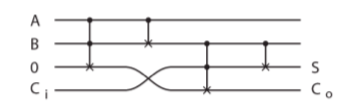
\includegraphics[scale=0.6]{full-adder.png}
\end{center}

In the figure (copied from a more general paper that includes
alternative designs~\cite{Rentergem2005OptimalDO}), the full adder
takes 4 inputs: the two bits to add $A$ and $B$, an incoming carry bit
$C_i$, and a heap input initialized to 0 to maintain
reversibility. There are four outputs: the first two are identical to
the incoming bits $A$ and $B$ and are considered ``garbage.'' The
third bit $S$ is the sum and the last bit $C_o$ is the outgoing carry
bit. In the notation used to describe the circuit, the $x$ denotes
boolean negation, the dots are control bits. In our reversible
language, we can express this circuit as the following permutation of
type $[2^4] \rightarrow [2^4]$:

\[\begin{array}{ll}
\mathit{swap}~12~14 \fatsemi \mathit{swap}~13~15 & \mbox{toffoli} \\
\mathit{swap}~8~12 \fatsemi \mathit{swap}~9~14 \fatsemi 
    \mathit{swap}~10~13 \fatsemi \mathit{swap}~11~15 & \mbox{cnot and swap} \\
\mathit{swap}~6~7 \fatsemi \mathit{swap}~14~15 & \mbox{toffoli} \\
\mathit{swap}~4~6 \fatsemi \mathit{swap}~5~7 \fatsemi
    \mathit{swap}~12~14 \fatsemi \mathit{swap}~13~15 & \mbox{cnot}
\end{array}\]

Note how the implementation of $\mathit{cnot}$ as a permutation
$[2^2] \rightarrow [2^2]$ cannot be directly reused in a circuit
$[2^4] \rightarrow [2^4]$. Indeed, in programming practice we are
interested in structured data and compositional abstractions which
will be the subject on next section. What we do learn however from
this short investigation using untyped flat sets is what the
``\emph{purely operational}'' view of the theory would be. In
particular, it tells us that permutations are an inescapable part of
the fabric of reversible computing.  However as permutations are
untyped, and act on the canonicalized version of $n$-element sets
(i.e. those sets where all the structure has been forgotten), these
are a rather pale shadow of the rich tapestry of
information-perserving transformations of structured data which we
investigate next.

%%%%%%%%%%%%%%%%%%%%%%%%%%%%%%%%%%%%%%%%%%%%%%%%%%%%%%%%%%%%%%%%%
\section{Data II: Structured Finite Types}

Instead of spaces consisting solely of unstructured isolated points,
we now investigate structured spaces built from sums and products of
elementary spaces. This structure corresponds to the building blocks
of type theory which are: the empty type ($\bot$), the unit type
($\top$), the sum type ($\uplus$), and the product ($\times$)
type. Before getting into the formal theory, let's consider possible
deformations on the space
$(\top \uplus \bot) \times (\top \uplus \top)$. This space is the
product of two subspaces: the subspace $(\top \uplus \bot)$ which
itself is the sum of the space $\top$ containing one element
$\texttt{tt}$ and the empty space $\bot$ and the subspace
$(\top \uplus \top)$ which is the sum of two spaces each containing
the one element $\texttt{tt}$. First, as discussed in the previous
section, any deformation of this space must at least preserve the
number of elements: we can neither create nor destroy points during
any continuous deformation. Seeing that the number of elements in our
example space is 2, a reasonable hypothesis is that we can deform the
space above to any other space with 2 elements such as
$\top \uplus \top$ or $\top \uplus (\top \uplus \bot)$. What this
really means is that we are treating the sum and product structure as
malleable. For example, imagining a product structure as arranged in a
grid, by stretching we can turn this structure to a sum structure
arranged in a line, change the orientation of the grid by exchanging
the axes, as well as do other transformations to be discussed in this
section that preserve the number of points.

%%%%%%%%%
\subsection{A Model of Type Equivalences} 

We now turn into the mathematical formalization of this idea. Our goal
is a denotational semantics on types that maintains the number of
points. First we note that the type structure of types has a nice
correspondence (Curry-Howard) to logic:

\begin{center}
\begin{tabular}{c|c}
Logic & Types \\ \hline
$\false$ & $\bot$ \\
$\true$ & $\top$ \\
$\land$ & $\times$ \\
$\lor$ & $\uplus$ \\
\end{tabular}
\end{center}

\noindent This correspondence is rather fruitful. As logical
expressions form a commutative semiring, we would expect that types
too form a commutative semiring. And indeed they do -- at least up to
\emph{type isomorphism}.  The natural numbers $\Nat$ are another
commutative semiring; it will turn out that, even though the
Curry-Howard correspondence has been extremely fruitful for
programming language research, it is $\Nat$ which will be a better
model for finite structured types as the corresponding commutative
semiring captures the familiar numerical identities that preserve the
number of points in the types.

\begin{defn}
\label{def:rig}
A \emph{commutative semiring} (sometimes called a \emph{commutative
  rig} (commutative ri\emph{n}g without negative elements)
$(R,0,1,+,\cdot)$ consists of a set $R$, two distinguished elements of
$R$ named 0 and 1, and two binary operations~$+$ and $\cdot$,
satisfying the following relations for any $a,b,c \in R$:
\[\begin{array}{rcl}
0 + a &=& a \\
a + b &=& b + a \\
a + (b + c) &=& (a + b) + c \\
\\
1 \cdot a &=& a \\
a \cdot b &=& b \cdot a \\
a \cdot (b \cdot c) &=& (a \cdot b) \cdot c \\
\\
0 \cdot a &=& 0 \\
(a + b) \cdot c &=& (a \cdot c) + (b \cdot c)
\end{array}\]
\end{defn}

\begin{prop}
The structure $\left(\mathbb{B}, \false, \true, \lor, \land\right)$
is a commutative semiring.
\end{prop}

We would like to adapt the commutative semiring definition to the
setting of structured types. First, types do not naturally want to be
put together into a ``set''.  This can be fixed if we replace the set
$R$ with a universe $U$, and replace the set membership $0 \in R$ with
the typing judgement $\bot : U$ (and similarly for the other
items). Our next instinct would be to similarly replace $=$ with a
judgement $A \equiv B$ that asserts that $A$ and $B$ are
\emph{propositionally equal}. This is however not true: the
proposition $A \times B \equiv B \times A$ is not
normally\footnote{Except In homotopy type theory where equivalent
  types are identified.} provable for arbitrary types $A$ and $B$. But
it should be clear that $A \times B$ and $B \times A$ contain
equivalent information. In other words, we would like to be able to
witness that $A \times B$ can be reversibly deformed into
$B \times A$. Which motivates the introduction of type
\emph{equivalences}. To do this, we need a few important auxiliary
concepts.

\begin{defn}[Homotopy]
\label{def:homotopy}
Two functions $f,g:A \rightarrow B$ are \emph{homotopic} if
$\forall x:A. f(x) \equiv g(x)$. We denote this $f \sim g$.
\end{defn}

\noindent It is easy to prove that homotopies (for any given function
space $A \rightarrow B$) are an equivalence relation.  The simplest
definition of the data which makes up an equivalence is the following.

\begin{defn}[Quasi-inverse]
\label{def:quasi}
For a function $f : A \rightarrow B$, a \emph{quasi-inverse} is a
triple $(g, \alpha, \beta)$, consisting of a function
$g : B \rightarrow A$ and two homotopies
$\alpha : f \circ g \sim \mathrm{id}_B$ and
$\beta : g \circ f \sim \mathrm{id}_A$.
\end{defn}

\begin{defn}[Equivalence of types]
  Two types $A$ and $B$ are equivalent $A \simeq B$ if there exists a
  function $f : A \rightarrow B$ together with a quasi-inverse for $f$.
\end{defn}

\noindent Why \emph{quasi}? The reasons are beyond our scope, but the
interested reader can read Sec.~$2.4$ and Ch.~$4$ in the HoTT
book~\cite{hottbook}.  There are several conceptually different, but
equivalent, ``better'' definitions.  We record just one here:

\begin{defn}[Bi-invertibility]
\label{def:biinv}
For a function $f : A \rightarrow B$, a \emph{bi-inverse} is a
pair of functions $g,h : B \rightarrow A$ and two homotopies
$\alpha : f \circ g \sim \mathrm{id}_B$ and
$\beta : h \circ f \sim \mathrm{id}_A$.
\end{defn}

\noindent We can then replace quasi-inverse with bi-invertibility in
the definition of type equivalence. The differences will not matter to
us here.

We are now in position to formally state the appropriate commutative
semiring structure for types. After replacing the set $R$ with a
universe $U$, we also replace the algebraic use of $=$ in
Def.~\ref{def:rig} by the type equivalence relation $\simeq$. With
this change, we can indeed prove that types (with
$\bot, \top, \uplus, \times$) form a commutative semiring. The reader
familiar with universal algebra should pause and ponder a bit about
what we have done. We have lifted \emph{equality} from being in the
signature of the ambient logic and instead put it in the signature of
the algebraic structure of interest. Then, and only then, are we in a
solid position to show that we have a concept (commutative semiring)
which is flexible enough for types to be an instance.

If we revisit the Curry-Howard correspondence, we notice one
more issue. In logic, it is true that $A \lor A = A$ and
$A \land A = A$. However, neither $A \uplus A$ nor $A \times A$ are
equivalent to $A$. They are however \emph{equi-inhabited}. This is
a fancy way of saying
\[ A \uplus A \ \text{is inhabited} \qquad \Leftrightarrow \qquad A \
  \text{is inhabited} \] The above is the real \textit{essence} of the
Curry-Howard correspondence.  In other words, classical Curry-Howard
tells us about \emph{logical equivalence} of types. This is even a
constructive statement: there are indeed functions
$f : A \uplus A \rightarrow A$ and $g : A \rightarrow A \uplus A$;
however, they are not inverses.

So mere inhabitation falls far short of our goals of being able to
smoothly deform from one type to another. Let us thus analyze the crux
of the ``problem''. In logic, we have that $\land$ and $\lor$ are both
\emph{idempotent}: this is the property of any binary operation $*$
where $\forall a. a * a = a$. And it should be clear that an
idempotent operations is a \emph{forgetful} operation: its input has
two copies of $a$, but its output, only one. On the type side,
something more subtle happens. Consider $\top \uplus \top$
versus $\top$; the first has \emph{two} proofs of inhabitation
($\texttt{inl tt}$ and $\texttt{inr tt}$) while the second only one
($\texttt{tt}$). These cannot be put in bijective correspondence. Even
though the ``payload'' \texttt{tt} is the same, forgetting
$\texttt{inl}$ (or \texttt{inr}) throws away information -- something
we have expressly disallowed.  Yes, this should remind you of
Maxwell's demon: even though the data is the same, they are tagged
differently, and this data is indeed information, and must be
preserved.

\begin{figure}[t]
\[
\begin{array}{rrcll}
\idc :& A & \simeq & A &: \idc \\
\\
\identlp :&  \bot \uplus A & \simeq & A &: \identrp \\
\swapp :&  A \uplus B & \simeq & B \uplus A &: \swapp \\
\assoclp :&  A \uplus (B \uplus C) & \simeq & (A \uplus B) \uplus C &: \assocrp \\
\\
\identlt :&  \top \times A & \simeq & A &: \identrt \\
\swapt :&  A \times B & \simeq & B \times A &: \swapt \\
\assoclt :&  A \times (B \times C) & \simeq & (A \times B) \times C &: \assocrt \\
\\
\distz :&~ \bot \times A & \simeq & \bot ~ &: \factorzl \\
\dist :&~ (A \uplus B) \times C & \simeq & (A \times C) \uplus (B \times C)~ &: \factor
\end{array}
\]
\caption{Type isomorphisms.}
\label{type-isos}
\end{figure}

Nevertheless, the Curry-Howard correspondence still has some force. We
know that the inhabitants of types formed with with
$\bot, \top, \uplus, \times$ are a commutative semiring. What we want
to know is, which types are equivalent? From a commutative semiring
perspective, this amounts to asking what terms are equal?  We have a
set of generators for those equations, namely those in
Def.~\ref{def:rig}. What we thus need is to create $8$ pairs of
mutually inverse functions which witness these identities.  For
concreteness, we show the signatures in Fig.~\ref{type-isos}.  As
these all come in symmetric pairs (some of which are self-symmetric),
we give names for both directions. 

%%%%%%%%%
\subsection{A Language of Type Equivalences} 

\begin{figure}[t]
\[
\begin{array}{rrcll}
\idc :& \tau & \iso & \tau &: \idc \\
\\
\identlp :&  0 + \tau & \iso & \tau &: \identrp \\
\swapp :&  \tau_1 + \tau_2 & \iso & \tau_2 + \tau_1 &: \swapp \\
\assoclp :&  \tau_1 + (\tau_2 + \tau_3) & \iso & (\tau_1 + \tau_2) + \tau_3 &: \assocrp \\
\\
\identlt :&  1 * \tau & \iso & \tau &: \identrt \\
\swapt :&  \tau_1 * \tau_2 & \iso & \tau_2 * \tau_1 &: \swapt \\
\assoclt :&  \tau_1 * (\tau_2 * \tau_3) & \iso & (\tau_1 * \tau_2) * \tau_3 &: \assocrt \\
\\
\distz :&~ 0 * \tau & \iso & 0 ~ &: \factorzl \\
\dist :&~ (\tau_1 + \tau_2) * \tau_3 & \iso & (\tau_1 * \tau_3) + (\tau_2 * \tau_3)~ &: \factor
\end{array}
\]
\caption{$\Pi$-terms.}
\label{pi-terms}
\end{figure}

We now have in our hands our desired denotational semantics. We want
to create a programming language, which we call $\Pi$, such that the
types and type combinators map to $\bot, \top, \uplus, \times$, and
such that we have ground terms whose denotation are all $16$ type
isomorphisms of Fig.~\ref{type-isos}. This is completely
straightforward, as we can simply do this literally. To make the
analogy with commutative semirings stand out even more, we will use
$0, 1, +$, and $\times$ at the type level, and will denote
``equivalence'' by $\iso$.  Thus Fig.~\ref{pi-terms} shows the
``constants'' of the language. Note how we have continued with
the spirit of Curry-Howard: the terms of $\Pi$ are \emph{proof terms},
but rather than being witnesses of inhabitation, they are witnesses of
equivalences. Thus the proof language of commutative semiring equivalences
becomes terms of $\Pi$.

\begin{figure}[t]
\[
\Rule{}
{\jdg{}{}{c_1 : \tau_1 \iso \tau_2} \quad \vdash c_2 : \tau_2 \iso \tau_3}
{\jdg{}{}{c_1 \odot c_2 : \tau_1 \iso \tau_3}}
{}
\qquad
\Rule{}
{\jdg{}{}{c_1 : \tau_1 \iso \tau_2} \quad \vdash c_2 : \tau_3 \iso \tau_4}
{\jdg{}{}{c_1 \oplus c_2 : \tau_1 + \tau_3 \iso \tau_2 + \tau_4}}
{}
\]
\[
\Rule{}
{\jdg{}{}{c_1 : \tau_1 \iso \tau_2} \quad \vdash c_2 : \tau_3 \iso \tau_4}
{\jdg{}{}{c_1 \otimes c_2 : \tau_1 * \tau_3 \iso \tau_2 * \tau_4}}
{}
\]
\caption{$\Pi$-combinators.}
\label{pi-combinators}
\end{figure}

Of course, one does not get a programming language with just typed
constants! There is a need to perform multiple equivalences. There are
in fact three ways to do this: sequential composition $\odot$, choice
composition $\oplus$ (sometimes called juxtaposition), and parallel
composition $\otimes$. See Fig.~\ref{pi-combinators} for the
signatures. The construction $c_1 \odot c_2$ corresponds to performing
$c_1$ first, then $c_2$, and is the usual notion of composition -- and
corresponds to $\fatsemi$ of the language of permutations of
Sec.~\ref{sec:dataone}. The construction $c_1 \oplus c_2$ chooses to
perform $c_1$ or $c_2$ depending on whether the input is labelled
$\textsf{inl}$ or $\textsf{inr}$ respectively. Finally the
construction $c_1 \otimes c_2$ operates on a product structure, and
applies $c_1$ to the first component and $c_2$ to the second.

The type-erase of this language \emph{should} be permutations. But
given types $A$ and $B$ that erase to $\fin{m}$ and $\fin{n}$ respectively,
what are $A + B$ and $A * B$ ?  They correspond exactly to
$\fin{m+n}$ and $\fin{m*n}$!  Geometrically, this corresponds to
concatenation for $A + B$, i.e. lining up the elements of $A$ first,
and then those of $B$. For $A * B$, one can picture this as
lining up the elements of $A$ horizontally, those of $B$ vertically
and perpendicular to those of $A$, and filling in the square with
pairs of elements from $A$ and $B$; if one re-numbers these sequentially,
reading row-wise, this gives an enumeration of $\fin{m*n}$.

From here, it is easy to see what, for example, $c_1 \oplus c_2$ must be,
operationally: from a permutation on $\fin{m}$ and another on $\fin{n}$,
create a permutation on $\fin{m+n}$ by having $c_1$ operate on the first
$m$ elements of $A+B$, and $c_2$ operate on the last $n$ elements. 
Similarly, $\swapp$ switches the roles of $A$ and $B$, and thus corresponds
to $\fin{n+m}$. Note how we ``recover'' the commutativity of 
natural number addition from this type isomorphism. Geometrically, $\swapt$
is also rather interesting: it corresponds to matrix transpose!
Furthermore, in this representations, some combinators like
$\identlp$ and $\assoclp$ are identity operations: the underlying representations
are not merely isomorphic, they are definitionally equal.
In other words, the passage to $\Nat$ erases some structural information.

\jc{it would be nice to have a picture or two here}

Embedded in our definition of $\Pi$ is a design decision: to make the
terms of $\Pi$ \emph{syntactically} reversible. In other words, to
every $\Pi$ constant, there is another $\Pi$ constant which is its
inverse. This is not the only choice.  Another would be to add a
$\mathit{flip}$ combinator to the language; we could then remove
quite a few combinators as redundant. The drawback is that many
programs in $\Pi$ become longer. Furthermore, some of the symmetry
at ``higher levels'' (see next section) is also lost. Since the
extra burden of language definition and of proofs is quite low, we
prefer the structural symmetry over a minimalistic language definition.

\jc{We should decide what you level convention is. Do we say
that $\iso$ is level 0, so that $\Leftrightarrow$ is level 1?
We need to be consistent about it.}

\jc{wavefront}

sound and complete isomorphisms for finite types

\begin{verbatim}
examples:
  (1 + 1) x ((1 + 1) x b) = (b+b) + (b+b)
  conditionals
  toffoli
  fredkin
\end{verbatim}

\begin{figure}[t]
Let $c_1 : t_1 \leftrightarrow t_2$,  $c_2 : t_2 \leftrightarrow t₃$, and $c_3 : t_3 \leftrightarrow t_4$:
\[\def\arraystretch{1.3}
\begin{array}{c}
  {c_1 \odot (c_2 \odot c_3) \Leftrightarrow (c_1 \odot c_2) \odot c_3}
\\
  {(c_1 \oplus (c_2 \oplus c_3)) \odot \assoclp \Leftrightarrow \assoclp \odot ((c_1 \oplus c_2) \oplus c_3)}
\\
  {(c_1 \otimes (c_2 \otimes c_3)) \odot \assoclt \Leftrightarrow \assoclt \odot ((c_1 \otimes c_2) \otimes c_3)}
\\
  {((c_1 \oplus c_2) \oplus c_3) \odot \assocrp \Leftrightarrow \assocrp \odot (c_1 \oplus (c_2 \oplus c_3))}
\\
  {((c_1 \otimes c_2) \otimes c_3) \odot \assocrt \Leftrightarrow \assocrt \odot (c_1 \otimes (c_2 \otimes c_3))}
\\
  {\assocrp \odot \assocrp \Leftrightarrow ((\assocrp \oplus \idc) \odot \assocrp) \odot (\idc \oplus \assocrp)}
\\
  {\assocrt \odot \assocrt \Leftrightarrow ((\assocrt \otimes \idc) \odot \assocrt) \odot (\idc \otimes \assocrt)}
\end{array}\]
\caption{\label{figj}Signatures of level-1 $\Pi$-combinators: associativity}
\end{figure}

\begin{figure}[t]
Let $a : t_1 \leftrightarrow t_2$, $b : t_3 \leftrightarrow t_4$, and $c : t₅ \leftrightarrow t₆$:
\[\def\arraystretch{1.3}
\begin{array}{c}
  {((a \oplus b) \otimes c) \odot \dist \Leftrightarrow \dist \odot ((a \otimes c) \oplus (b \otimes c))}
\\
  {(a \otimes (b \oplus c)) \odot \distl \Leftrightarrow \distl \odot ((a \otimes b) \oplus (a \otimes c))}
\\
  {((a \otimes c) \oplus (b \otimes c)) \odot \factor \Leftrightarrow \factor \odot ((a \oplus b) \otimes c)}
\\
  {((a \otimes b) \oplus (a \otimes c)) \odot \factorl \Leftrightarrow \factorl \odot (a \otimes (b \oplus c))}
\end{array}\]
\caption{\label{figi}Signatures of level-1 $\Pi$-combinators: distributivity and factoring}
\end{figure}

\begin{figure}[t]
Let $c, c_1, c_2, c_3 : t_1 \leftrightarrow t_2$ and $c', c'' : t_3 \leftrightarrow t_4$:
\[\def\arraystretch{1.3}
\begin{array}{c}
  {\idc \odot \, c \Leftrightarrow c}
\quad
  {c \, \odot \idc \, \Leftrightarrow c}
\quad
  {c\,\, \odot\,! c \Leftrightarrow \idc}
\quad
  {! c \odot c \Leftrightarrow \idc}
\\
  {c \Leftrightarrow c}
\quad
\Rule{}
  {c_1 \Leftrightarrow c_2 \quad c_2 \Leftrightarrow c_3}
  {c_1 \Leftrightarrow c_3}
  {}
\quad
\Rule{}
  {c_1 \Leftrightarrow c' \quad c_2 \Leftrightarrow c''}
  {c_1 \odot c_2 \Leftrightarrow c' \odot c''}
  {}
\end{array}\]
\caption{\label{figh}Signatures of level-1 $\Pi$-combinators: identity and composition}
\end{figure}

\begin{figure}[t]
Let $c₀ : 0 \leftrightarrow 0$, $c_1 : 1 \leftrightarrow 1$, and $c : t_1 \leftrightarrow t_2$:
\[\def\arraystretch{1.3}
\begin{array}{c}
  {\identlp \odot c \Leftrightarrow (c₀ \oplus c) \odot \identlp}
\qquad
  {\identrp \odot (c₀ \oplus c) \Leftrightarrow c \odot \identrp}
\\
  {\identlsp \odot c \Leftrightarrow (c \oplus c₀) \odot \identlsp}
\qquad
  {\identrsp \odot (c \oplus c₀) \Leftrightarrow c \odot \identrsp}
\\
  {\identlt \odot c \Leftrightarrow (c_1 \otimes c) \odot \identlt}
\qquad
  {\identrt \odot (c_1 \otimes c) \Leftrightarrow c \odot \identrp}
\\
  {\identlst \odot c \Leftrightarrow (c \otimes c_1) \odot \identlst}
\qquad
  {\identrst \odot (c \otimes c_1) \Leftrightarrow c \odot \identrst}
\\
  {\identlt \Leftrightarrow \distl \odot (\identlt \oplus \identlt)}
\\
\identlp \Leftrightarrow \swapp \odot \identrsp
\qquad
\identlt \Leftrightarrow \swapt \odot \identrst
\end{array}\]
\caption{\label{figg}Signatures of level-1 $\Pi$-combinators: unit}
\end{figure}

\begin{figure}[t]
Let $c_1 : t_1 \leftrightarrow t_2$ and $c_2 : t_3 \leftrightarrow t_4$:
\[\def\arraystretch{1.3}
\begin{array}{c}
  {\swapp \odot (c_1 \oplus c_2) \Leftrightarrow (c_2 \oplus c_1) \odot \swapp}
\quad
  {\swapt \odot (c_1 \otimes c_2) \Leftrightarrow (c_2 \otimes c_1) \odot \swapt}
\\
  {(\assocrp \odot \swapp) \odot \assocrp \Leftrightarrow ((\swapp \oplus \idc) \odot \assocrp) \odot (\idc \oplus \swapp)}
\\
  {(\assoclp \odot \swapp) \odot \assoclp \Leftrightarrow ((\idc \oplus \swapp) \odot \assoclp) \odot (\swapp \oplus \idc)}
\\
  {(\assocrt \odot \swapt) \odot \assocrt \Leftrightarrow ((\swapt \otimes \idc) \odot \assocrt) \odot (\idc \otimes \swapt)}
\\
  {(\assoclt \odot \swapt) \odot \assoclt \Leftrightarrow ((\idc \otimes \swapt) \odot \assoclt) \odot (\swapt \otimes \idc)}
\end{array}\]
\caption{\label{figf}Signatures of level-1 $\Pi$-combinators: commutativity and associativity}
\end{figure}

\begin{figure}[t]
Let $c_1 : t_1 \leftrightarrow t_2$, $c_2 : t_3 \leftrightarrow t_4$, $c_3 : t_1 \leftrightarrow t_2$, and $c_4 : t_3 \leftrightarrow t_4$. \\
Let $a_1 : t₅ \leftrightarrow t_1$,  $a_2 : t₆ \leftrightarrow t_2$, $a_3 : t_1 \leftrightarrow t_3$, and $a_4 : t_2 \leftrightarrow t_4$.
\[\def\arraystretch{1.3}
\begin{array}{c}
\Rule{}
  {c_1 \Leftrightarrow c_3 \quad c_2 \Leftrightarrow c_4}
  {c_1 \oplus c_2 \Leftrightarrow c_3 \oplus c_4}
  {}
\qquad
\Rule{}
  {c_1 \Leftrightarrow c_3 \quad c_2 \Leftrightarrow c_4}
  {c_1 \otimes c_2 \Leftrightarrow c_3 \otimes c_4}
  {}
\\
  {\idc \oplus \, \idc \, \Leftrightarrow \idc}
\qquad
  {\idc \otimes \, \idc \, \Leftrightarrow \idc}
\\
  {(a_1 \odot a_3) \oplus (a_2 \odot a_4) \Leftrightarrow (a_1 \oplus a_2) \odot (a_3 \oplus a_4)}
\\
  {(a_1 \odot a_3) \otimes (a_2 \odot a_4) \Leftrightarrow (a_1 \otimes a_2) \odot (a_3 \otimes a_4)}
\end{array}\]
\caption{\label{fige}Signatures of level-1 $\Pi$-combinators: functors}
\end{figure}

\begin{figure}[t]
\[\def\arraystretch{1.3}
\begin{array}{c}
  {\identlsp \oplus \idc ~\Leftrightarrow~ \assocrp \odot (\idc \oplus \, \identlp)}
\\
  {\identlst \otimes \idc ~\Leftrightarrow~ \assocrt \odot (\idc \otimes \, \identlt)}
\end{array}\]
\caption{\label{figd}Signatures of level-1 $\Pi$-combinators: unit and associativity}
\end{figure}


\begin{figure}[t]
Let $c : t_1 \leftrightarrow t_2$:
\[\def\arraystretch{1.3}
\begin{array}{c}
  {(c \otimes \idc) \odot \absorbl \Leftrightarrow \absorbl \odot \idc}
\quad
  {(\idc \, \otimes c) \odot \absorbr \Leftrightarrow \absorbr \odot \idc}
\\
  {\idc \odot \, \factorzl \Leftrightarrow \factorzl \odot (\idc \otimes c)}
\quad
  {\idc \odot \, \factorzr \Leftrightarrow \factorzr \odot (c \otimes \idc)}
\\
  {\absorbr \Leftrightarrow \absorbl}
\\
  {\absorbr \Leftrightarrow (\distl \odot (\absorbr \oplus \absorbr)) \odot \identlp}
\\
  {\identlst \Leftrightarrow \absorbr}
\qquad
  {\absorbl \Leftrightarrow \swapt \odot \absorbr}
\\
  {\absorbr \Leftrightarrow (\assoclt \odot (\absorbr \otimes \idc)) \odot \absorbr}
\\
  {(\idc \otimes \absorbr) \odot \absorbl \Leftrightarrow (\assoclt \odot (\absorbl \otimes \idc)) \odot \absorbr}
\\
  {\idc \otimes \, \identlp \Leftrightarrow (\distl \odot (\absorbl \oplus \idc)) \odot \identlp}
\end{array}\]
\caption{\label{figc}Signatures of level-1 $\Pi$-combinators: zero}
\end{figure}

\begin{figure}[t]
\[\def\arraystretch{1.3}
\begin{array}{c}
  {((\assoclp \otimes \idc) \odot \dist) \odot (\dist \oplus \idc) \Leftrightarrow (\dist \odot (\idc \oplus \dist)) \odot \assoclp}
\\
  {\assoclt \odot \distl \Leftrightarrow ((\idc \otimes \distl) \odot \distl) \odot (\assoclt \oplus \assoclt)}
\end{array}\]
\vspace{ -0.5em}
\[\def\arraystretch{1.3}
\begin{array}{rcl}
  (\distl \odot (\dist \oplus \dist)) \odot \assoclp &\Leftrightarrow&
   \dist \odot (\distl \oplus \distl) \odot \assoclp ~\odot \\
&& (\assocrp \oplus \idc) ~\odot \\
&& ((\idc \oplus \swapp) \oplus \idc) ~\odot \\
&&      (\assoclp \oplus \idc)
\end{array}\]
\caption{\label{figb}Signatures of level-1 $\Pi$-combinators: associativity and distributivity}
\end{figure}

\begin{figure}[t]
\[\def\arraystretch{1.3}
\begin{array}{rcl}
  (\idc \otimes \swapp) \odot \distl &\Leftrightarrow& \distl \odot \swapp
\\
  \dist \odot (\swapt \oplus \swapt) &\Leftrightarrow & \swapt \odot \distl
\end{array}\]
\caption{\label{figa}Signatures of level-1 $\Pi$-combinators: commutativity and distributivity}
\end{figure}

Implement Fredkin gate and mention the following:

\begin{quote}
  Ed Fredkin pursued the idea that information must be finite in
  density. One day, he announced that things must be even more simple
  than that. He said that he was going to assume that information
  itself is conserved. “You’re out of you mind, Ed.” I
  pronounced. “That’s completely ridiculous. Nothing could happen in
  such a world. There couldn’t even be logical gates. No decisions
  could ever be made.” But when Fredkin gets one of his ideas, he’s
  quite immune to objections like that; indeed, they fuel him with
  energy. Soon he went on to assume that information processing must
  also be reversible — and invented what’s now called the Fredkin
  gate. (Minsky 1999)
\end{quote}

%%%%%%%%%%%%%%%%%%%%%%%%%%%%%%%%%%%%%%%%%%%%%%%%%%%%%%%%%%%%%%%%%
\section{Data III: Reversible Programs between Reversible Programs}

In the previous sections, we examined equivalences between
conventional data structures, i.e, sets of values and structured trees
of values. We now consider a richer, less conventional, but
foundational notion of data: programs themselves. Indeed, universal
computation models fundamentally rely on the fact that \emph{programs
are (or can be encoded as) data}, e.g., a Turing machine can be
encoded as a string that another Turing machine (or even the same
machine) can manipulate. In our setting, the programs developed in the
previous section are reversible deformations between structured finite
types. We now ask whether these programs can themselves
be subject to (higher-level) reversible deformations?

Before developing the theory, let's consider a small example
consisting of two deformations between the types $A + B$ and $C+D$:

\begin{center}
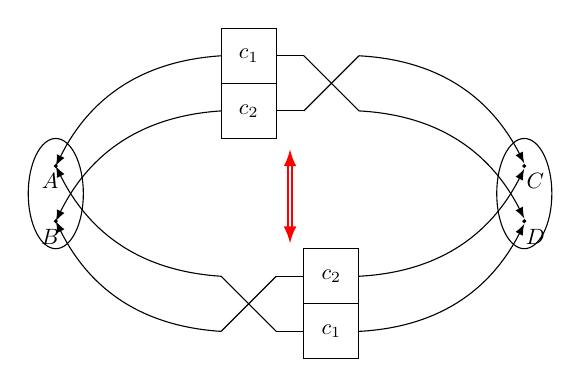
\begin{tikzpicture}[scale=0.7,every node/.style={scale=0.8}]
  \draw[>=latex,<->,double,red,thick] (2.25,-1.2) -- (2.25,-2.9) ;
%%  \node at (3.3,-2) {$\mathit{swapl}_{+\Leftrightarrow}$} ;
%%  \node at (2.5,-1.3) {$((c_2~\oplus~c_1)~\odot~\mathit{swap}_{+})$};
%%  \node at (2.5,-2.7) {$(\mathit{swap}_{+}~\odot~(c_1~\oplus~c_2))$};
  \draw (-2,-2) ellipse (0.5cm and 1cm);
  \draw[fill] (-2,-1.5) circle [radius=0.025];
  \node[below] at (-2.1,-1.5) {$A$};
  \draw[fill] (-2,-2.5) circle [radius=0.025];
  \node[below] at (-2.1,-2.5) {$B$};

  \draw (6.5,-2) ellipse (0.5cm and 1cm);
  \draw[fill] (6.5,-1.5) circle [radius=0.025];
  \node[below] at (6.7,-1.5) {$C$};
  \draw[fill] (6.5,-2.5) circle [radius=0.025];
  \node[below] at (6.7,-2.5) {$D$};

  \draw[<-] (-2,-1.5) to[bend left] (1,0.5) ;
  \draw[<-] (-2,-2.5) to[bend left] (1,-0.5) ;
  \draw[->] (3.5,0.5) to[bend left] (6.5,-1.45) ;
  \draw[->] (3.5,-0.5) to[bend left] (6.5,-2.45) ;

  \draw[<-] (-2,-1.5) to[bend right] (1,-3.5) ;
  \draw[<-] (-2,-2.5) to[bend right] (1,-4.5) ;
  \draw[->] (3.5,-3.5) to[bend right] (6.5,-1.55) ;
  \draw[->] (3.5,-4.5) to[bend right] (6.5,-2.55) ;

  \draw     (2.5,-3)  -- (3.5,-3) -- (3.5,-4) -- (2.5,-4) -- cycle ;
  \draw     (2.5,-4)  -- (3.5,-4) -- (3.5,-5) -- (2.5,-5) -- cycle ;

  \draw     (1,1)  -- (2,1) -- (2,0) -- (1,0) -- cycle ;
  \draw     (1,0)  -- (2,0) -- (2,-1) -- (1,-1) -- cycle ;

  \node at (3,-3.5) {$c_2$};
  \node at (3,-4.5) {$c_1$};

  \node at (1.5,0.5) {$c_1$};
  \node at (1.5,-0.5) {$c_2$};

  \draw     (2,0.5)  -- (2.5,0.5)  ;
  \draw     (2,-0.5) -- (2.5,-0.5) ;

  \draw     (2.5,0.5)  -- (3.5,-0.5)  ;
  \draw     (2.5,-0.5) -- (3.5,0.5) ;

  \draw     (1,-3.5)  -- (2,-4.5)    ;
  \draw     (1,-4.5) -- (2,-3.5)   ;

  \draw     (2,-3.5)  -- (2.5,-3.5)    ;
  \draw     (2,-4.5) -- (2.5,-4.5)   ;

\end{tikzpicture}
\end{center}
The top path is the $\Pi$ program
$(c_1~\oplus~c_2)~\odot~\swapp$ which deforms the
type $A$ by $c_1$, deforms the type $B$ by $c_2$, and deforms the
resulting space by a twist that exchanges the two injections into the
sum type. The bottom path performs the twist first and then deforms
the type $A$ by $c_1$ and the type $B$ by $c_2$ as before. If one
could imagine the paths are physical wires and the deformations $c_1$
and $c_2$ as arbitrary deformations on these wires then, holding the
points $A$, $B$, $C$, and $D$ fixed, it is possible to rotate the top
part of the diagram to become identical to the bottom one. That
rotation can be undone (reversed), which takes the bottom
part of the diagram into the top part.  In other
words, there exists a deformation of the program
$(c_1~\oplus~c_2)~\odot~\swapp$ to the program
$\swapp \odot (c_2~\oplus~c_1)$. We can also show that this
means that, as permutations, $(c_1~\oplus~c_2)~\odot~\swapp$ and
$\swapp \odot (c_2~\oplus~c_1)$ are equal. And, of course, not
all programs between the same types can be deformed into one
another. The simplest example of inequivalent deformations
are the two automorphisms of $1+1$, namely $\idc$ and $\swapp$.

In the previous section, we saw how we could take the proof
terms of commutative semirings as our starting point. What we need
now is to understand how proofs of algebraic identities should be
considered equivalent. Classical algebra does not help, as proofs
in algebra are not considered first-class citizens. However,
another route is available to us: since the work of 
Hofmann and Streicher~\cite{hofmann96thegroupoid}, we know that
one can model types as \emph{groupoids}.  Previously, we
modeled types as (finite) sets.

Thus, rather than looking at (untyped) commutative semirings,
we should looked at a \emph{typed} version. This process frequently
goes by the moniker of ``categorification''.  We want a categorical
algebra, where the basic objects are groupoids (to model our types),
and where there is a natural notion of $+$ and $*$.  At first,
we hit what seems like a serious stumbling block: the category of
all groupoids, Groupoid, does not have co-products or products.
We don't want to work internally in Groupoid -- we want operations
\emph{on} groupoids. In other words, we want something akin to
symmetric monoidal categories, but with two interacting 
monoidal structures.  Luckily, this already exists: the categorical
analog to (commutative) semirings are (symmetric) Rig Categories.
This straightforwardly generalizes to symmetric Rig Groupoids.

How does this help? Coherence conditions! Symmetric monoidal categories,
to start somewhere simple, do not just introduce weak transformations
like the associator $\alpha$ and the left $\lambda$ and right $\rho$
unitors, but also coherence conditions that these must satisfy. Looking,
for example, at just the additive fragment of $\Pi$ (i.e. with just $0$,
$1$ and $+$ for the types, $\odot$ and $\oplus$ as combinators, and
only the terms so expressible), the sub-language would correspond,
denotationally, to exactly symmetric monoidal groupoids. And what
these possess are exactly some \emph{equations between equations}
as commutative diagrams.  Adding in the coherence conditions 
corresponding to naturality of the various transformers gives us a
list of equations between programs.  Furthermore, the natural transformations
that arise are in fact natural isomorphisms -- all of which are
reversible.

We can then proceed to prove that every one of the coherence conditions
involved in defining a symmetric Rig Groupoid holds for the groupoid
interpretation of types.

\amr{*** another wavefront ***}

Pi level 2.

So we end up looking, semantically, at weak Rig Groupoid. Syntactically,
we take the easiest way there: simply make every coherence isomorphism into
a combinator. Huge proof obligation that this induces actual transformations
on Pi programs. Luckily, it does.  But not straightforwardly -- ``incorrect''
definitions of some Pi combinators (such as those for 0*x = 0) can lead to
some level 2 morphisms not working.

The interpretation on permutations is unclear, because the Pi representation
has so much more structure, and permutations too have many different
representations. So it is unclear what maps to what.

%%%%%%%%%%%%%%%%%%%%%%%%%%%%%%%%%%%%%%%%%%%%%%%%%%%%%%%%%%%%%%%%%
\section{Data IV: Circle ???}

Would be interesting

%%%%%%%%%%%%%%%%%%%%%%%%%%%%%%%%%%%%%%%%%%%%%%%%%%%%%%%%%%%%%%%%%
\section{Conclusion}

Discuss recursion, or add a section of infinite sets???

CS abstractions are based on ``old'' physics

computer applications are more and more ``physical''

physical principles such as conservation of information should be part
of our foundational abstractions

quest for other principles; other data models; graphs; HoTT

Data IV: Recursive Types

Add recursion to structured finite types, trace, feedback, loop...

Natural numbers: fold/unfold

Partial isos

meta-circular interpreter

DANGER: here, we leave the safe land of ``preservation of information'',
because partiality is not reversible. So while trace gives a reversible
program as output, it itself isn't a reversible operation. Like the
demon's brain in Maxwell's thought experiment, trace irreversible work!
So trace, which is fundamental to all work with recursive types, is
only reversible "at level 1". So we need to replace trace with some other
operation for level 2 reversibility to also hold -- and this is an open
problem.

Data V: Exclusive Disjunctions

Quantum over finite field

\jc{The reason I commented this out is that it is under-justified. The
reader will simply not understand what these next few lines are really
saying.}
Indeed one should take the physical principles underlying quantum mechanics,
the most successful physical theory known to us and adapt computation to
``learn'' from these principles. To illustrate the depth of our crisis, Scott
Aaronson, Umesh Vazirani, and others have proposed the following puzzle.

One of these wild claims must be true!:
\begin{itemize}
\item the extended Church-Turing thesis is false, or
\item quantum physics is false, or
\item there is an efficient classical algorithm for factoring
\end{itemize}
Indeed, if quantum physics is correct then there is an efficient quantum
algorithm for factoring (Shor). If there is no efficient classical algorithm
for factoring then the extended Church-Turing thesis is false.

%% Below are pieces of text that are not immediately useful above, but
%% from which we might still be able to pilfer usefully.

%%%%%%%%%
\subsection{Technical Overview}

The technical development derives from ideas which are implicit in the
works of \cite{toffoli:1980, Zuliani:2001:LR,
  malacaria2007assessing,ClarkHM07,Ghica:2007:GSS:1190216.1190269}.
(1) Functions whose output entropy is equal to their input entropy are
information preserving functions.  (2) A function
$f : b_1 \rightarrow b_2$ is \emph{logically reversible} if there
exists an inverse function $f^{\dagger}$ such that for any input
$v_1:b_1$ if there exists $v_2:b_2$ such that $f(v_1)=v_2$ \emph{iff}
$f^{\dagger}(v_2)=v_1$.  (3) Logically reversible functions are
information preserving.

To summarize:
\begin{enumerate}
\item Based on isomorphisms of sum and product
  types~\cite{Fiore:2004}, we develop a strong normalizing model of
  computing, which we call $\Pi$, that is logically reversible and
  information preserving. Every computation expressible in $\Pi$
  is an isomorphism.

\item We extend $\Pi$ with isorecursive type and trace operators from
  category theory to obtain $\Pi$. Every computation expressible in
  $\Pi$ is a partial isomorphism --- i.e. the system admits
  non-termination. $\Pi$ is Turing complete while being information
  preserving and logically reversible.

\item We develop the categorical semantics of these
  models~\cite{rc2011}. \amr{Mention n-categories.} We also develop
  a graphical notation for programming in these models that
  reminiscent of Penrose diagrams for
  categories~\cite{selinger-graphical}, Geometry of Interaction (GoI)
  machines and Proof
  Nets~\cite{Mackie2011,DBLP:conf/popl/Mackie95}. In the graphical
  notation, computation is modeled by the flow of particles in a
  circuit.

\item Since these new models are substantially different from \lcal\
  or familiar high-level languages, a point of concern is how one can
  effectively develop programs in them.  We address this by presenting
  a straightforward technique for deriving $\Pi$ programs by
  systematically translating logically reversible small-step abstract
  machines~\cite{isoint}. Complex programs can be devised in this way;
  we demonstrate the derivation of a meta-circular interpreter for
  $\Pi$.

\item We develop an arrow meta-language to encapsulate information
  effects. This metalanguage serves to encapsulate effects, in much
  the same way that traditional arrows or monads serve to encapsulate
  effects over the \lcal.

\item We show how a conventional irreversible model can be expressed
  in our model. We compile the first-order fragment of typed \lcal\
  extended with sums, products and loops to $\Pi$. This compilation is
  interesting for two reasons: (1) it exposes the implicit information
  effects of \lcal\ in the compilation to $\Pi$ and (2) the
  compilation of $\Pi$ to $\Pi$ shows that information effects can be
  erased by treating them as interactions with an explicit information
  environment.

\item We develop the notion of `duality' in $\Pi$ which gives us not
  one duality (like in linear logic or Filinski's symmetric
  \lcal~\cite{Filinski:89}), but two notions of duality -- an additive
  duality and a multiplicative duality. This gives a crisp semantics
  for negative and fractional types in the context of $\Pi$.

\end{enumerate}

Several intriguing areas of exploration remain and the book concludes
with discussion of some of these, along with other possible
applications.  Of these, the field of reversible and Quantum computing
is closely related and we survey several connections in depth.  The
exact connection between $\Pi$ and linear logic~\cite{Girard87tcs} is
not fully understood though it is clear that both systems capture
related but different notions of resource usage. A closely related
area is the connection with duality of computation \cite{Filinski:89,
  DBLP:conf/icfp/CurienH00, 10.1109/LICS.2010.23,Wadler:2003} ---
i.e., the quest for a unifying framework between `computations',
values, continuations and their logical counterparts. The
investigation of duality gives rise to negative and fractional types
which have an intuitive semantics and are reminiscent of negative
information flow, superposition and entanglement from Quantum
Physics~\cite{piee}.

%%%%%%%%%
\paragraph*{Conservation of Information.}

If information has a physical significance, then it is subject to
conservation laws just as mass and energy are.  To make this idea
concrete and to provide a taste of the applications it opens, consider
a tiny 2-bit password = \verb|"10"|. The password checker looks like:

% verbatim for now, will go to something decent later
\begin{verbatim}
check-password (guess) =
  if guess == "10"
  then True
  else False
\end{verbatim}

One can ask how much information is leaked by this program assuming
the attacker has no prior knowledge except that the password is 2
bits, i.e., the four possible 2-bits are equally likely. If the
attacker guesses \verb|"10"| (with probability $1/4$) the password (2
bits) is leaked. If the attacker guesses one of the other choices
(with probability $3/4$) the number of possibilities is reduced from 4
to 3, i.e., the attacker learns $\log{4} - \log{3}$ bits of
information. So in general the attacker learns\footnote{If the
  password is 8 restricted ASCII characters (6 bits), the attacker
  learns 0.00001 bits in the first probe.}:
\[\begin{array}{ll}
   &  1/4 * 2 + 3/4 (\log{4} - \log{3}) \\
  =&  1/4 \log{4} + 3/4 \log{4/3} \\
  =&  - 1/4 \log{1/4} - 3/4 \log{3/4} \\
  \sim& 0.8 \mbox{~bits~in~the~first~probe}
\end{array}\]

One can alternatively look at the situation by viewing the input as a
random variable with 4 possibilities and a uniform distribution (i.e.,
with 2 bits of information). The output is another random variable
with 4 possibilities but with the distribution
$\{ (True, 1/4), (False, 3/4) \}$ which contains 0.8 bits of
information. Thus 2 input bits of information were given to the
function and only 0.8 were produced. Where did the 1.2 bits of
information go? Once we accept the thesis that information is a
physical entity this question cannot be ignored.

The Landauer Principle states that erasing information requires
energy. In other words, the password checking function must have
erased 1.2 bits during its calculation, which dissipate as heat in any
physical realization of the function. In conventional models of
computation, this erasure is \emph{implicit}, i.e., it occurs as a
side effect of calculation. We wish to look at models where
erasure is simply not allowed.

There are, in fact, many different principles of physics which are at
odds with our current models of computation. Even within quantum
mechanics itself, there are other ideas (such as superposition or
entanglement) which are not present in current models. We will however
restrict ourselves to exploring a single dimension in which our
foundations should be revised: \textbf{conservation of information}.
We will follow its consequences, which will turn out to be far
reaching.

\begin{quote}
  The laws of physics are essentially algorithms for calculation. These
  algorithms are significant only to the extent that they are executable in
  our real physical world. Our usual laws of physics depend on the
  mathematician's real number system. With that comes the presumption that
  given any accuracy requirement, there exist a number of calculations steps,
  which if executed, will satisfy that accuracy requirement. But the real
  world is unlikely to supply us with unlimited memory of unlimited Turing
  machine tapes, Therefore, continuum mathematics is not executable, and
  physical laws which invoke that can not really be satisfactory. They are
  references to illusionary procedures. Rolf Landauer, The physical nature of
  information, Physics Letters A 217 (1996) pp. 188-193:
\end{quote}

A high level approach to conservation of information would proceed
as follows:
\begin{enumerate}
\item Create a means to measure information.
\item Show that this measure is sound with respect to our current understanding
of what information ought to be.
\item Assert that whatever ``quantity'' of information a system has, must
remain invariant throughout the lifetime of the system.
\end{enumerate}

Certainly, whatever our notion of information, it can neither be created,
duplicated, nor erased. Of course, if we make our notion of information
too rigid, it will be impossible to even \textbf{modify} it! For computation
to occur, modification must be possible.  But of what kind?

\amr{We should also have a quick survey of other works in reversible
computation? Most of the other work tries to start from well known
models of computation or well known programming languages, and then
adapts them to be reversible. Pi is different in that it starts from
the semantic implications of reversibility. Then, because it adds
types, rather than control-flow (or even data-flow) as its next layer
of ``understanding'', this leads to equivalences, isomorphisms, etc.
This then leads, quite naturally, to finding that the ``proof
language'' of semirings (and Rig Groupoids at level 2) is actually a
programming language. And it is Pi. This is a neat twist on
Curry-Howard because CH is about \textbf{inhabitation} only. But with
``conservation of information'' as the basis, a different kind of
correspondence arises; in fact, this one may well be an actual
isomorphism.}

%%%%%%%%%
\paragraph*{Information.}
We can now give a first precise definition of information preservation.
Let
`$b$' be a (not necessarily finite) type whose values are labeled
$b^1, b^2, \ldots$. Let $\xi$ be a random variable of type $b$ that is
equal to $b^i$ with probability $p_i$. The entropy of $\xi$ is defined
as $-\sum p_i \log{p_i}$~\cite{Shannon1948}.  Consider a function
$f : b_1 \rightarrow b_2$ where $b_2$ is a (not necessarily finite)
type whose values are labeled $b_2^1, b_2^2, \ldots$. The output
entropy of the function is given by $- \sum q_j \log{q_j}$ where $q_j$
indicates the probability of the output of the function to have value
${b_2}^j$. We say a function is \emph{information-preserving} if its
output entropy is equal to the entropy of its input. In later sections,
we will refine this view.

\amr{
Talk about conservation of information in biology, computer science,
evolutionary computing, and search. (See
\url{http://www.evolutionnews.org/2012/08/conservation_of063671.html}.
}

In our current age, both Landauer's Principle and recent investigations
of computational models well-suited to quantum mechanics, push us to
revisit our current models of computation. Information, on top of
having a physical manifestation, appears to be \emph{conserved},
along with other quantities like energy, mass and momentum.

But what does it mean for a computation to preserve information?
What is the missing principle that will guide the creation of a new
model of computation that ``conserve information''?
It is nature to look again at physics for inspiration --
in our current understanding of physics all of the primitive rules
are reversible. Conventional computation is not. Can
we embrace this simple principle as the building block of a model of
computation? What would computation look like when viewed from this
vantage point? Can non-trivial computation be performed in a
reversible manner? And, if so, does it have applications?

Traditional models of computation are all unityped, generally
operating on unstructured sequences of symbols. But recent
investigations, in the intersection between mathematics and
computer science (particularly in Homotopy Type Theory~\cite{hottbook})
reveal that not only can mathematics be typed, but that doing so
reveals further structure -- in both mathematics and in computation.

And that brings us to the principal objective of this survey: explore the
domain of \emph{typed reversible computation}.

\amr{In the quantum case, this is clear. Say something about topological
quantum computing.}

\textbf{punch line: allowable operations that computers can perform
  while embracing the laws of physics are operations that preserve
  everthing in abstract space of ``data''; doughnut into cup kind of
  transformations.}

%%%%%%%%%%%%%%%%%%%%%%%%%%%%%%%%%%%%%%%%%%%%%%%%%%%%%%%%%%%%%%%%%
\section{Theseus: Types and Simple Isomorphisms}
\label{theseusI}

We begin by presenting the core of Theseus which consists of evidently
reversible functions on user-defined datatypes.  In subsequent discourse we
will use the word `map' to refer to these logically reversible
functions. Theseus has the same built-in types as~\ensuremath{\Pi^{o}} and as conventional
functional programming languages: the empty type, the unit type, and sum and
product types. All other types, including recursive types, are user-defined
using a general mechanism for type declarations:

\lstset{
        language=haskell,
 morekeywords={Bool,Nat,Tree},
	keywordstyle=\bfseries\ttfamily,
	identifierstyle=\ttfamily,
	commentstyle=\ttfamily,
	stringstyle=\ttfamily,
	showstringspaces=false,
	basicstyle=\scriptsize\sffamily,
	tabsize=2,
	breaklines=false,
	breakatwhitespace=false,
	aboveskip={1.2\baselineskip},
        columns=fixed,
        extendedchars=true,
}
\begin{lstlisting}[escapeinside={(@}{@)}]
type Bool  =  (@\ctr{True}@) | (@\ctr{False}@)
type Nat   =  0 | Succ Nat
type Tree  =  Leaf Nat | Node Tree Tree
 \end{lstlisting}
%subcode source theseus.tex:347

\noindent The declarations above witness isomorphisms between the set
\kw{Bool} and the set constructed by the constants \ctr{True} and
\ctr{False}, between the set \kw{Nat} and the set inductively constructed
using {\scriptsize{0}} and \ctr{Succ}, and between the set \kw{Tree} and the
set inductively constructed using \ctr{Leaf} and \ctr{Node}.  Thus, Theseus
type definitions are similar to, say, Haskell, type definitions. Such
definitions translate directly to the underlying \ensuremath{\Pi^{o}} using iso-recursive
type definitions. For example, the above types translate as follows:
\vspace{-20pt}
\begin{small}
\begin{multicols}{3}
\[\begin{array}{rclr}
\kw{Bool}   & = &  \mu  ~x.1 + 1 \\
\kw{Nat}   & = &  \mu  ~x. 1 + x \\
\kw{Tree}   & = &  \mu  ~x. \kw{Nat}  + x * x \\
 \end{array}\]
%subcode source theseus.tex:363

\[\begin{array}{rclr}
\mathit{unfoldBool} :& \kw{Bool}  \leftrightarrow 1 + 1 &: \mathit{foldBool} \\
\mathit{unfoldNat} :& \kw{Nat}  \leftrightarrow 1 + \kw{Nat}  &: \mathit{foldNat} \\
\mathit{unfoldTree} :& \kw{Tree}  \leftrightarrow \kw{Nat}  + (\kw{Tree}  * \kw{Tree} ) &: \mathit{foldTree} \\
 \end{array}\]
%subcode source theseus.tex:368
\end{multicols}
\end{small}

%%%%%%%%%%%%
\subsection{Simple Isomorphisms}

A Theseus program has a type of the form \ctr{a} $\leftrightarrow$ \ctr{b};
one runs such a program forward by supplying a value of type \ctr{a}. If the
program terminates, we get back a value of type~\ctr{b}. Alternately we can
run the program in reverse by supplying a value of type \ctr{b}. Given the
built-in types and the facility to introduce user-defined ones, one can
already write a few small but interesting programs. Maps that are evidently
isomorphisms can be written in the familiar pattern matching style
popularized by the family of functional languages. For example:
\begin{multicols}{2}
\lstset{
        language=haskell,
 morekeywords={Nat,Tree,Int,Bool},
	keywordstyle=\bfseries\ttfamily,
	identifierstyle=\ttfamily,
	commentstyle=\ttfamily,
	stringstyle=\ttfamily,
	showstringspaces=false,
	basicstyle=\scriptsize\sffamily,
	tabsize=2,
	breaklines=false,
	breakatwhitespace=false,
	aboveskip={1.2\baselineskip},
        columns=fixed,
        extendedchars=true,
}
\begin{lstlisting}[escapeinside={(@}{@)}]
(@\ctr{id}@) :: Bool (@$\leftrightarrow$@) Bool
| (@\ctr{False}@)  (@$\leftrightarrow$@)  (@\ctr{False}@)
| (@\ctr{True}@)   (@$\leftrightarrow$@)  (@\ctr{True}@)

expandBool :: Bool * a (@$\leftrightarrow$@) a + a
| (@\ctr{True}@), a   (@$\leftrightarrow$@)  (@\ctr{Left}@) a
| (@\ctr{False}@), a  (@$\leftrightarrow$@)  (@\ctr{Right}@) a

expandNat :: Nat (@$\leftrightarrow$@) Nat + 1
| 0       (@$\leftrightarrow$@)  (@\ctr{Right}@) ()
| Succ n  (@$\leftrightarrow$@)  (@\ctr{Left}@) n

(@\ctr{not}@) :: Bool (@$\leftrightarrow$@) Bool
| (@\ctr{True}@)   (@$\leftrightarrow$@)  (@\ctr{False}@)
| (@\ctr{False}@)  (@$\leftrightarrow$@)  (@\ctr{True}@)

foldBool :: a + a (@$\leftrightarrow$@) Bool * a
| (@\ctr{Left}@) a   (@$\leftrightarrow$@)  (@\ctr{True}@), a
| (@\ctr{Right}@) a  (@$\leftrightarrow$@)  (@\ctr{False}@), a

foldNat :: Nat + 1 (@$\leftrightarrow$@) Nat
| (@\ctr{Right}@) ()  (@$\leftrightarrow$@)  0
| (@\ctr{Left}@) n    (@$\leftrightarrow$@)  Succ n
 \end{lstlisting}
%subcode source theseus.tex:410
\end{multicols}

\vspace{-25pt}
\lstset{
        language=haskell,
 morekeywords={Nat,Tree,Int,Bool},
	keywordstyle=\bfseries\ttfamily,
	identifierstyle=\ttfamily,
	commentstyle=\ttfamily,
	stringstyle=\ttfamily,
	showstringspaces=false,
	basicstyle=\scriptsize\sffamily,
	tabsize=2,
	breaklines=false,
	breakatwhitespace=false,
	aboveskip={1.2\baselineskip},
        columns=fixed,
        extendedchars=true,
}
\begin{lstlisting}[escapeinside={(@}{@)}]
treeUnwind :: Tree (@$\leftrightarrow$@) Tree * Tree + (Bool + Nat)
| Node t1 t2            (@$\leftrightarrow$@)  (@\ctr{Left}@)   (t1, t2)
| Leaf 0                (@$\leftrightarrow$@)  (@\ctr{Right}@)  ((@\ctr{Left}@) (@\ctr{True}@))
| Leaf (Succ 0)         (@$\leftrightarrow$@)  (@\ctr{Right}@)  ((@\ctr{Left}@) (@\ctr{False}@))
| Leaf (Succ (Succ n))  (@$\leftrightarrow$@)  (@\ctr{Right}@)  ((@\ctr{Right}@) n)
 \end{lstlisting}
%subcode source theseus.tex:422

Unlike the situation in a conventional functional language, the
intuition here is that the two sides of each pattern clause can be
swapped to produce the inverse of the function, i.e. as we will see
repeatedly in the paper, patterns and expressions are the same
thing. Compare for example the definitions of \ctr{expandBool} and
\ctr{foldBool}. This is the only constraint that a programmer needs to
maintain. This constraint can be ensured using the following two
rules:

\begin{enumerate}
\label{rules}
\item \emph{Non-overlapping and exhaustive coverage in pattern
  clauses.} The collections of patterns in the left-hand side (LHS) of
  each clause must be a complete non-overlapping covering of the input
  type. Similarly, the collections of patterns in the right-hand side
  (RHS) of each clause must also be a complete non-overlapping
  covering of the return type. In other words, no cases should be
  omitted or duplicated.
\item \emph{Preserve typed variables across \ensuremath{\leftrightarrow}.} Each variable that
  occurs on one side of a pattern matching clause can only appear once on
  that side and must appear exactly once on the other side and with the same
  type.
\end{enumerate}

When restricted to one side of each pattern matching clause, the rules
should be familiar and intuitive. Note that, in general, the two sides
of a pattern matching clause may have different types. Other than the
requirement of non-overlapping and exhaustive coverage, there are no
rules that constrain the types and names of constants nor of
constructors. So for example, in \ctr{foldBool}, the pattern
`\ctr{Left}~\ctr{a}' maps to a pair constructor with the first
component being the constant \ctr{True}.

Examples of expressions that violate the constraints follow:

\begin{multicols}{2}
\lstset{
        language=haskell,
 morekeywords={Nat,Tree,Int,Bool},
	keywordstyle=\bfseries\ttfamily,
	identifierstyle=\ttfamily,
	commentstyle=\ttfamily,
	stringstyle=\ttfamily,
	showstringspaces=false,
	basicstyle=\scriptsize\sffamily,
	tabsize=2,
	breaklines=false,
	breakatwhitespace=false,
	aboveskip={1.2\baselineskip},
        columns=fixed,
        extendedchars=true,
}
\begin{lstlisting}[escapeinside={(@}{@)}]
-- Invalid: Missing LHS cases
missing_node :: Tree (@$\leftrightarrow$@) Nat
| Leaf n (@$\leftrightarrow$@) n

-- Invalid: Overlapping RHS cases
overlapping_cases :: Nat (@$\leftrightarrow$@) Nat
| 0       (@$\leftrightarrow$@)  0
| Succ n  (@$\leftrightarrow$@)  n
 \end{lstlisting}
%subcode source theseus.tex:471

\lstset{
        language=haskell,
 morekeywords={Nat,Tree,Int,Bool},
	keywordstyle=\bfseries\ttfamily,
	identifierstyle=\ttfamily,
	commentstyle=\ttfamily,
	stringstyle=\ttfamily,
	showstringspaces=false,
	basicstyle=\scriptsize\sffamily,
	tabsize=2,
	breaklines=false,
	breakatwhitespace=false,
	aboveskip={1.2\baselineskip},
        columns=fixed,
        extendedchars=true,
}
\begin{lstlisting}[escapeinside={(@}{@)}]
-- Invalid: n is dropped
drop_var :: Tree (@$\leftrightarrow$@) Tree * Tree + Nat
| Node t1 t2  (@$\leftrightarrow$@)  (@\ctr{Left}@)  (t1,t2)
| Leaf n      (@$\leftrightarrow$@)  (@\ctr{Right}@) 0

-- Invalid: t is used twice
dup_var :: Tree (@$\leftrightarrow$@) Tree * Tree + Nat
| Node t t  (@$\leftrightarrow$@)  (@\ctr{Left}@)  (t,t)
| Leaf n    (@$\leftrightarrow$@)  (@\ctr{Right}@) n
 \end{lstlisting}
%subcode source theseus.tex:485
\end{multicols}

\noindent It is easy to see that every primitive isomorphism of \ensuremath{\Pi^{o}} can
be expressed in Theseus. Here are a few examples.
\vspace{-10pt}
\begin{multicols}{2}
\lstset{
        language=haskell,
 morekeywords={Nat,Tree,Int,Bool},
	keywordstyle=\bfseries\ttfamily,
	identifierstyle=\ttfamily,
	commentstyle=\ttfamily,
	stringstyle=\ttfamily,
	showstringspaces=false,
	basicstyle=\scriptsize\sffamily,
	tabsize=2,
	breaklines=false,
	breakatwhitespace=false,
	aboveskip={1.2\baselineskip},
        columns=fixed,
        extendedchars=true,
}
\begin{lstlisting}[escapeinside={(@}{@)}]
assocL :: a+(b+c) (@$\leftrightarrow$@) (a+b)+c :: assocR
| (@\ctr{Left}@) a          (@$\,\,\leftrightarrow$@) (@\ctr{Left}@) ((@\ctr{Left}@) a)
| (@\ctr{Right}@) ((@\ctr{Left}@) b)   (@$\leftrightarrow$@) (@\ctr{Left}@) ((@\ctr{Right}@) b)
| (@\ctr{Right}@) ((@\ctr{Right}@) c)  (@$\leftrightarrow$@) (@\ctr{Right}@) c
 \end{lstlisting}
%subcode source theseus.tex:499

\lstset{
        language=haskell,
 morekeywords={Nat,Tree,Int,Bool},
	keywordstyle=\bfseries\ttfamily,
	identifierstyle=\ttfamily,
	commentstyle=\ttfamily,
	stringstyle=\ttfamily,
	showstringspaces=false,
	basicstyle=\scriptsize\sffamily,
	tabsize=2,
	breaklines=false,
	breakatwhitespace=false,
	aboveskip={1.2\baselineskip},
        columns=fixed,
        extendedchars=true,
}
\begin{lstlisting}[escapeinside={(@}{@)}]
zeroe :: b + 0 (@$\leftrightarrow$@) b :: zeroi
| (@\ctr{Left}@) v (@$\leftrightarrow$@) v

swapTimes :: a * b (@$\leftrightarrow$@) b * a
| (a,b) (@$\leftrightarrow$@) (b,a)
 \end{lstlisting}
%subcode source theseus.tex:509
\end{multicols}

\label{translation}
\noindent
Every simple isomorphism of Theseus can be translated to \ensuremath{\Pi^{o}} as follows:
\begin{enumerate}
\item For every Theseus map \ctr{c : a} $\leftrightarrow$ \ctr{b}, we can
  define an intermediate type \ctr{ti} which is the sum of pairs of all the
  variables that occur in the LHS patterns. Since the LHS and RHS patterns
  contain the same type variables, \ctr{ti} is unique for a given \ctr{c} (up
  to ordering). For example, in \ctr{treeUnwind} the first clause has
  variables \lstinline{t1 : Tree} and \lstinline{t2 : Tree}, the second and
  third clauses have no variables and the fourth clause has the variable
  \lstinline{n : Nat}. The expected type \ctr{ti} is therefore
  \lstinline{Tree * Tree + (1 + (1 + Nat))}, where we insert the type
  {\scriptsize{1}} as a placeholder for the clauses that did not have type
  variables.
\item By construction \ctr{ti} is isomorphic to \ctr{a} and \ctr{b}. Hence,
  maps \ctr{c1 : a} $\leftrightarrow$ \ctr{ti} and \ctr{c2 : ti}
  $\leftrightarrow$ \ctr{b} must be expressible in \ensuremath{\Pi^{o}}. (Both the above
  isomorphisms can be constructed by systematically unfolding and
  distributing \ctr{a} and \ctr{b} until \ctr{ti} is obtained.  The exact
  details of such an expansion can be found in Sec.~3 of our previous
  paper~\cite{rc2012} and are skipped in this paper.) Once values of type
  \ctr{a} and \ctr{b} can be mapped to values of type \ctr{ti}, the required
  translation of \ctr{c} is given by \ctr{c1} $\fatsemi$ \ctr{c2}.
\end{enumerate}

%%%%%%%%%%%%
\subsection{Dealing with Numbers}

If we try to do arithmetic using the previously defined Peano-style \ensuremath{\kw{Nat} },
we have to address an issue of what to do when we encounter
\lstinline{sub1 0}. There are two obvious choices:
\begin{enumerate}
\item We can define \ctr{add1} and \ctr{sub1} of type \kw{Nat}
  $\leftrightarrow$ \kw{Nat}, such that \ctr{sub1} of {\scriptsize{0}}
  diverges. We show how these maps can be defined in Sec.~\ref{add1}.
\item An error mechanism can be added to the language such that when
  an error is raised program execution is undefined and there is no
  meaningful inverse definition.
\end{enumerate}
Another choice, similar to that made by Janus, is to use bounded integers
such that every operation is always well defined through underflows and
overflows. Here is a simple 4-bit \kw{Nat4} datatype with its corresponding
\ctr{add1} and \ctr{sub1} operations:
\lstset{
        language=haskell,
 morekeywords={Nat,Tree,Int,Bool,Nat4},
	keywordstyle=\bfseries\ttfamily,
	identifierstyle=\ttfamily,
	commentstyle=\ttfamily,
	stringstyle=\ttfamily,
	showstringspaces=false,
	basicstyle=\scriptsize\sffamily,
	tabsize=2,
	breaklines=false,
	breakatwhitespace=false,
	aboveskip={1.2\baselineskip},
        columns=fixed,
        extendedchars=true,
}
\begin{lstlisting}[escapeinside={(@}{@)}]
type Nat4 = Bool * Bool * Bool * Bool

add1 :: Nat4 (@$\leftrightarrow$@) Nat4 :: sub1
| (a, b, c, (@\ctr{False}@))          (@$\leftrightarrow$@)  (a, b, c, (@\ctr{True}@))
| (a, b, (@\ctr{False}@), (@\ctr{True}@))       (@$\,\leftrightarrow$@)  (a, b, (@\ctr{True}@), (@\ctr{False}@))
| (a, (@\ctr{False}@), (@\ctr{True}@), (@\ctr{True}@))    (@$\,\,\leftrightarrow$@)  (a, (@\ctr{True}@), (@\ctr{False}@), (@\ctr{False}@))
| ((@\ctr{False}@), (@\ctr{True}@), (@\ctr{True}@), (@\ctr{True}@))  (@$\leftrightarrow$@)  ((@\ctr{True}@), (@\ctr{False}@), (@\ctr{False}@), (@\ctr{False}@))
| ((@\ctr{True}@), (@\ctr{True}@), (@\ctr{True}@), (@\ctr{True}@))   (@$\leftrightarrow$@)  ((@\ctr{False}@), (@\ctr{False}@), (@\ctr{False}@), (@\ctr{False}@))
 \end{lstlisting}
%subcode source theseus.tex:567

\noindent It is easy to see how a math library may be defined in this
way. Once an operator can be defined in Theseus it is always possible to
replace its implementation by an equivalent one that is expressible
efficiently in the underlying hardware. In this case one could compile down
to the CPU's native integer representation and operators.

%%%%%%%%%%%%%%%%%%%%%%%%%%%%%%%%%%%%%%%%%%%%%%%%%%%%%%%%%%%%%%%%%%%%%%%%%%%%%%
\section{Parametrized Maps}
\label{theseusII}

Now that we can express simple standalone isomorphisms, we explain how to
compose such isomorphisms to model more complex behavior. In \ensuremath{\Pi^{o}}, there
are three ways of composing isomorphisms: sequential composition, parallel
composition, and choice composition. The common idiom underlying these
composition combinators is that a reversible map can be parametrized by
another reversible map. This idea is related to ``higher-order functions''
but is more limited as we explain below.

%%%%%%%%%%%%
\subsection{Definition and Examples}

A Theseus map \ctr{f} can be parametrized by another map \ctr{g} by adding a
labeled argument~\ctr{g} of the appropriate type to \ctr{f}. In the example
below \ctr{treeUnwindf} is parametrized over some map \ctr{f} which it
applies to \ctr{n}, if the supplied tree is \lstinline{Leaf n}:
\lstset{
        language=haskell,
 morekeywords={Nat,Tree,Int,Bool},
	keywordstyle=\bfseries\ttfamily,
	identifierstyle=\ttfamily,
	commentstyle=\ttfamily,
	stringstyle=\ttfamily,
	showstringspaces=false,
	basicstyle=\scriptsize\sffamily,
	tabsize=2,
	breaklines=false,
	breakatwhitespace=false,
	aboveskip={1.2\baselineskip},
        columns=fixed,
        extendedchars=true,
}
\begin{lstlisting}[escapeinside={(@}{@)}]
treeUnwindf :: f:(Nat (@$\leftrightarrow$@) a) (@$\rightarrow$@) Tree (@$\leftrightarrow$@) Tree * Tree + a
| Node t1 t2 (@$\leftrightarrow$@) (@\ctr{Left}@) (t1, t2)
| Leaf n     (@$\leftrightarrow$@) (@\ctr{Right}@) (f n)
 \end{lstlisting}
%subcode source theseus.tex:600

\noindent This parametrization should be thought of as a macro or a
meta-language construction. Theseus does not have high-order maps in the
formal sense. In other words, the final type of a Theseus program must be of
the form \ctr{a} $\leftrightarrow$ \ctr{b} and every occurrence of an arrow
type $\rightarrow$ must be instantiated at compile time. The notation for
instantiating the label parameter \ctr{f} in the map \ctr{fun} by the map
\ctr{g} is \inline{fun}{f}{g}. For example,
\inline{treeUnwindf}{f}{expandNat} should be thought of as shorthand for the
map:
\lstset{
        language=haskell,
 morekeywords={Nat,Tree,Int,Bool},
	keywordstyle=\bfseries\ttfamily,
	identifierstyle=\ttfamily,
	commentstyle=\ttfamily,
	stringstyle=\ttfamily,
	showstringspaces=false,
	basicstyle=\scriptsize\sffamily,
	tabsize=2,
	breaklines=false,
	breakatwhitespace=false,
	aboveskip={1.2\baselineskip},
        columns=fixed,
        extendedchars=true,
}
\begin{lstlisting}[escapeinside={(@}{@)}]
_ :: Tree (@$\leftrightarrow$@) Tree * Tree + (1 + Nat)
| Node t1 t2    (@$\leftrightarrow$@) (@\ctr{Left}@) (t1, t2)
| Leaf 0        (@$\leftrightarrow$@) (@\ctr{Right}@) ((@\ctr{Right}@) ())
| Leaf (Succ n) (@$\leftrightarrow$@) (@\ctr{Right}@) ((@\ctr{Left}@) n)
 \end{lstlisting}
%subcode source theseus.tex:618

\noindent which inlines \ctr{expandNat} within the definition of
\ctr{treeUnwindf}.

We discuss the reversibility of parametrized maps in the next section. We
first point out that the \ensuremath{\Pi^{o}} closure primitives can be expressed as
parametrized maps:
\lstset{
        language=haskell,
	keywordstyle=\bfseries\ttfamily,
	identifierstyle=\ttfamily,
	commentstyle=\ttfamily,
	stringstyle=\ttfamily,
	showstringspaces=false,
	basicstyle=\scriptsize\sffamily,
	tabsize=2,
	breaklines=false,
	breakatwhitespace=false,
	aboveskip={1.2\baselineskip},
        columns=fixed,
        extendedchars=true,
}
\begin{lstlisting}[escapeinside={(@}{@)}]
_._ :: f:(a (@$\leftrightarrow$@) b) (@$\rightarrow$@) g:(b (@$\leftrightarrow$@) c) (@$\rightarrow$@) a (@$\leftrightarrow$@) c
| a (@$\leftrightarrow$@) g (f a)

_*_ :: f:(a (@$\leftrightarrow$@) b) (@$\rightarrow$@) g:(c (@$\leftrightarrow$@) d) (@$\rightarrow$@) a * c (@$\leftrightarrow$@) b * d
| (a,c) (@$\leftrightarrow$@) (f a , g c)

_+_ :: f:(a (@$\leftrightarrow$@) b) (@$\rightarrow$@) g:(c (@$\leftrightarrow$@) d) (@$\rightarrow$@) a + c (@$\leftrightarrow$@) b + d
| (@\ctr{Left}@) a   (@$\leftrightarrow$@)  (@\ctr{Left}@) (f a)
| (@\ctr{Right}@) c  (@$\leftrightarrow$@)  (@\ctr{Right}@) (g c)
 \end{lstlisting}
%subcode source theseus.tex:637

As an additional example, parametrized maps allow us to define controlled
operations in the tradition of reversible circuits. In the definition below,
the boolean input is a control bit that determines which of the maps \ctr{th}
or \ctr{el} is applied to the second component of the pair. This conditional
is then used to define the ``controlled-not'' gate:

\lstset{
        language=haskell,
	keywordstyle=\bfseries\ttfamily,
	identifierstyle=\ttfamily,
	commentstyle=\ttfamily,
	stringstyle=\ttfamily,
	showstringspaces=false,
	basicstyle=\scriptsize\sffamily,
	tabsize=2,
	breaklines=false,
	breakatwhitespace=false,
	aboveskip={1.2\baselineskip},
        columns=fixed,
        extendedchars=true,
}
\begin{lstlisting}[escapeinside={(@}{@)}]
(@\ctr{if}@) :: th:(a (@$\leftrightarrow$@) b) (@$\rightarrow$@) el:(a (@$\leftrightarrow$@) b) (@$\rightarrow$@) Bool * a (@$\leftrightarrow$@) Bool * b
| (@\ctr{True}@), a  (@$\leftrightarrow$@) (@\ctr{Left}@) (th a)
| (@\ctr{False}@), a (@$\leftrightarrow$@) (@\ctr{Right}@) (el a)

cnot :: Bool * Bool (@$\leftrightarrow$@) Bool * Bool
| control, bit (@$\leftrightarrow$@) if ~th:(@\ctr{not}@) ~el:(@\ctr{id}@) (control, bit)
 \end{lstlisting}
%subcode source theseus.tex:653

%%%%%%%%%%%%
\subsection{Reversing Parametrized Maps}

Reversing a map of type \ctr{a} $\leftrightarrow$ \ctr{b} results in a map of
type \ctr{b} $\leftrightarrow$ \ctr{a} which is its adjoint. As discussed
before, simple maps can be reversed by simply switching the LHS and RHS for
both the type and the pattern matching clauses comprising the
body. Interestingly, one can think about the reverse of parametrized maps in
the same way -- i.e. one simply needs to switch LHS and RHS of the `\ensuremath{\leftrightarrow}'.

\lstset{
        language=haskell,
 morekeywords={Nat,Tree,Int,Bool},
	keywordstyle=\bfseries\ttfamily,
	identifierstyle=\ttfamily,
	commentstyle=\ttfamily,
	stringstyle=\ttfamily,
	showstringspaces=false,
	basicstyle=\scriptsize\sffamily,
	tabsize=2,
	breaklines=false,
	breakatwhitespace=false,
	aboveskip={1.2\baselineskip},
        columns=fixed,
        extendedchars=true,
}
\begin{lstlisting}[escapeinside={(@}{@)}]
treeUnfold :: f:(Nat (@$\leftrightarrow$@) a) (@$\rightarrow$@) Tree (@$\leftrightarrow$@) Tree * Tree + a
| Node t1 t2  (@$\leftrightarrow$@) (@\ctr{Left}@) (t1, t2)
| Leaf n      (@$\leftrightarrow$@) (@\ctr{Right}@) (f n)

-- the adjoint of treeUnfold
rev_treeUnfold :: f:(Nat (@$\leftrightarrow$@) a) (@$\rightarrow$@) Tree * Tree + a (@$\leftrightarrow$@) Tree
| (@\ctr{Left}@) (t1, t2)  (@$\leftrightarrow$@) Node t1 t2
| (@\ctr{Right}@) (f n)    (@$\leftrightarrow$@) Leaf n
 \end{lstlisting}
%subcode source theseus.tex:676

\noindent Note that the application \lstinline{f n} happens on the left of
the \ensuremath{\leftrightarrow}, which is something that one does not see in conventional
functional languages. These applications in the LHS have the dual meaning of
applications in the RHS and should be understood as follows: the value that
is the actual argument of the \ctr{Right} constructor is the result of
applying~\lstinline{f n}. In the forward execution of
\lstinline{rev_treeUnfold}, when the actual value of the constructor argument
is encountered, it is passed through the reverse of \ctr{f} to get the value
\ctr{n}. In other words, the above program is exactly the same as
\lstinline{rev_treeUnfold'} below where \lstinline{rev_f} is the adjoint of
\ctr{f}:

\lstset{
        language=haskell,
 morekeywords={Nat,Tree,Int,Bool},
	keywordstyle=\bfseries\ttfamily,
	identifierstyle=\ttfamily,
	commentstyle=\ttfamily,
	stringstyle=\ttfamily,
	showstringspaces=false,
	basicstyle=\scriptsize\sffamily,
	tabsize=2,
	breaklines=false,
	breakatwhitespace=false,
	aboveskip={1.2\baselineskip},
        columns=fixed,
        extendedchars=true,
}
\begin{lstlisting}[escapeinside={(@}{@)}]
rev_treeUnfold' :: rev_f:(a (@$\leftrightarrow$@) Nat) (@$\rightarrow$@) Tree (@$\leftrightarrow$@) Tree * Tree + a
| (@\ctr{Left}@) (t1, t2) (@$\leftrightarrow$@) Node t1 t2
| (@\ctr{Right}@) a       (@$\leftrightarrow$@) Leaf (rev_f a)
 \end{lstlisting}
%subcode source theseus.tex:696

\noindent
It follows that the following programs are equivalent:
\vspace{-10pt}
\begin{multicols}{2}
\lstset{
        language=haskell,
 morekeywords={Nat,Tree,Int,Bool},
	keywordstyle=\bfseries\ttfamily,
	identifierstyle=\ttfamily,
	commentstyle=\ttfamily,
	stringstyle=\ttfamily,
	showstringspaces=false,
	basicstyle=\scriptsize\sffamily,
	tabsize=2,
	breaklines=false,
	breakatwhitespace=false,
	aboveskip={1.2\baselineskip},
        columns=fixed,
        extendedchars=true,
}
\begin{lstlisting}[escapeinside={(@}{@)}]
g :: f:(a (@$\leftrightarrow$@) b) (@$\rightarrow$@) a (@$\leftrightarrow$@) b
| a (@$\leftrightarrow$@) f a

g :: rev_f:(b (@$\leftrightarrow$@) a) (@$\rightarrow$@) a (@$\leftrightarrow$@) b
| rev_f b (@$\leftrightarrow$@) b
 \end{lstlisting}
%subcode source theseus.tex:710
\end{multicols}
\vspace{-15pt}
\noindent
Based on the above observation, it is easy to define the \ctr{sym} map that
constructs the adjoint of any given map:
\vspace{-5pt}
\lstset{
        language=haskell,
 morekeywords={Nat,Tree,Int,Bool},
	keywordstyle=\bfseries\ttfamily,
	identifierstyle=\ttfamily,
	commentstyle=\ttfamily,
	stringstyle=\ttfamily,
	showstringspaces=false,
	basicstyle=\scriptsize\sffamily,
	tabsize=2,
	breaklines=false,
	breakatwhitespace=false,
	aboveskip={1.2\baselineskip},
        columns=fixed,
        extendedchars=true,
}
\begin{lstlisting}[escapeinside={(@}{@)}]
sym :: f:(a (@$\leftrightarrow$@) b) (@$\rightarrow$@) b (@$\leftrightarrow$@) a
| (f a) (@$\leftrightarrow$@) a
 \end{lstlisting}
%subcode source theseus.tex:722
While parametrized maps add tremendous programming convenience to Theseus,
they don't change the expressive power of the language. All programs
expressible with parametrized maps, can be expressed without them by fully
inlining the actual parameters. Thus compiling Theseus programs with
parametrized maps to \ensuremath{\Pi^{o}} simply requires first inlining the maps and then
doing the translation described in Sec.~\ref{translation}.

%%%%%%%%%%%%%%%%%%%%%%%%%%%%%%%%%%%%%%%%%%%%%%%%%%%%%%%%%%%%%%%%%%%%%%%%%%%%%%
\section{Iteration Labels}
\label{theseusIII}
\label{add1}

The fragment of Theseus discussed up to now, modulo full recursive types, can
be expressed in pure \ensuremath{\Pi } without \ensuremath{\mathit{trace}}.  Introducing recursive
definitions in a reversible language is subtle because every iteration must
be reversible which requires, at least, that the number of iterations be
recoverable from the output. The insight we use in Theseus is that this can
be achieved elegantly by adding \emph{typed labels} as explained below. We
start with a small example:

\lstset{
        language=haskell,
 morekeywords={iter,Nat},
	keywordstyle=\bfseries\ttfamily,
	identifierstyle=\ttfamily,
	commentstyle=\ttfamily,
	stringstyle=\ttfamily,
	showstringspaces=false,
	basicstyle=\scriptsize\sffamily,
	tabsize=2,
	breaklines=false,
	breakatwhitespace=false,
	aboveskip={1.2\baselineskip},
        columns=fixed,
        extendedchars=true,
}
\begin{lstlisting}[escapeinside={(@}{@)}]
parity :: Nat * Bool (@$\leftrightarrow$@) Nat * Bool
| n, b                (@$\leftrightarrow$@) iter $ n, 0, b
| iter $ Succ n, m, b (@$\leftrightarrow$@) iter $ n, Succ m, (@\ctr{not}@) b
| iter $ 0, m, b      (@$\leftrightarrow$@) m, b
  where iter :: Nat * Nat * Bool
 \end{lstlisting}
%subcode source theseus.tex:751

\noindent The map \ctr{parity} calculates whether the given natural number is
even or odd by counting to {\scriptsize{0}} and flipping the second boolean
input each time. In the definition above, the label appears twice on the LHS
and twice on the RHS. The correctness (i.e., reversibility) of the map is
guaranteed as labels obey the same restrictions as the one for simple
patterns. In particular the occurrences of the label in the LHS must
constitute a non-overlapping coverage of the label type, and similarly for
the occurrences of the label in the RHS.

The important thing to note about labels is that they may have a
different type from the LHS or RHS types of their containing map. In
this case for example, the \ctr{parity} map has \lstinline{Nat * Bool}
as its LHS and RHS type while the type of the label \kw{iter} has the
type \lstinline{Nat * Nat * Bool}. Labels temporarily give us a
different \emph{view}~\cite{Wadler:1987:VWP:41625.41653} of a value,
by changing it type. Labels act as goto statements from one side to
the other -- when a label is encountered on the RHS of a map, the
argument to the label is matched by some definition of the label
pattern on the LHS of the map, and vice versa.  Here is a trace of the
execution of \ctr{parity} as it transforms input \ctr{Succ (Succ (Succ
  0)), False} to the output \ctr{Succ (Succ (Succ 0)), True}. It takes
five pattern match and rewrite steps to complete.

\lstset{
        language=haskell,
 morekeywords={iter,Nat},
	keywordstyle=\bfseries\ttfamily,
	identifierstyle=\ttfamily,
	commentstyle=\ttfamily,
	stringstyle=\ttfamily,
	showstringspaces=false,
	basicstyle=\scriptsize\sffamily,
	tabsize=2,
	breaklines=false,
	breakatwhitespace=false,
	aboveskip={1.2\baselineskip},
        columns=fixed,
        extendedchars=true,
}
\begin{lstlisting}[escapeinside={(@}{@)}]
Succ (Succ (Succ 0)), False           (@$\longmapsto$@) iter $ Succ (Succ (Succ 0)), 0, False
iter $ Succ (Succ (Succ 0)), 0, False (@$\longmapsto$@) iter $ Succ (Succ 0), Succ 0, True
iter $ Succ (Succ 0), Succ 0, True    (@$\longmapsto$@) iter $ Succ 0, Succ (Succ 0), False
iter $ Succ 0, Succ (Succ 0), False   (@$\longmapsto$@) iter $ 0, Succ (Succ (Succ 0)), True
iter $ 0, Succ (Succ (Succ 0)), True  (@$\longmapsto$@) Succ (Succ (Succ 0)), True
 \end{lstlisting}
%subcode source theseus.tex:784

A trace operator can be expressed using labels and the definition closely
follows the expected iteration semantics of \ensuremath{\mathit{trace}} in our previous
work~\cite{James:2012:IE:2103656.2103667}.  Using \ctr{trace} one can define
\ctr{add1} on \kw{Nat} such that \ctr{sub1} of {\scriptsize{0}}
diverges.

\begin{multicols}{2}
\lstset{
        language=haskell,
 morekeywords={enter,leave},
	keywordstyle=\bfseries\ttfamily,
	identifierstyle=\ttfamily,
	commentstyle=\ttfamily,
	stringstyle=\ttfamily,
	showstringspaces=false,
	basicstyle=\scriptsize\sffamily,
	tabsize=2,
	breaklines=false,
	breakatwhitespace=false,
	aboveskip={1.2\baselineskip},
        columns=fixed,
        extendedchars=true,
}
\begin{lstlisting}[escapeinside={(@}{@)}]
trace :: f:(a + b (@$\leftrightarrow$@) a + c) (@$\rightarrow$@) b (@$\leftrightarrow$@) c
| b               (@$\leftrightarrow$@) enter $ (@\ctr{Right}@) b
| enter $ a       (@$\leftrightarrow$@) leave $ (f a)
| leave $ (@\ctr{Left}@) a  (@$\leftrightarrow$@) enter $ (@\ctr{Left}@) a
| leave $ (@\ctr{Right}@) c (@$\leftrightarrow$@) c
  where enter :: a + b
        leave :: a + c
 \end{lstlisting}
%subcode source theseus.tex:803

\lstset{
        language=haskell,
 morekeywords={Nat},
	keywordstyle=\bfseries\ttfamily,
	identifierstyle=\ttfamily,
	commentstyle=\ttfamily,
	stringstyle=\ttfamily,
	showstringspaces=false,
	basicstyle=\scriptsize\sffamily,
	tabsize=2,
	breaklines=false,
	breakatwhitespace=false,
	aboveskip={1.2\baselineskip},
        columns=fixed,
        extendedchars=true,
}
\begin{lstlisting}[escapeinside={(@}{@)}]
addSub :: Nat + Nat (@$\leftrightarrow$@) Nat + Nat
| (@\ctr{Left}@) (Succ n) (@$\leftrightarrow$@) (@\ctr{Left}@) n
| (@\ctr{Left}@) 0        (@$\leftrightarrow$@) (@\ctr{Right}@) 0
| (@\ctr{Right}@) n       (@$\leftrightarrow$@) (@\ctr{Right}@) (Succ n)

add1 :: Nat (@$\leftrightarrow$@) Nat :: sub1
| n (@$\leftrightarrow$@) trace ~f:addSub n
 \end{lstlisting}
%subcode source theseus.tex:815
\end{multicols}
\vspace{-10pt}

Here are a few more examples that use labels.  Combinators \ctr{iterN} and
\ctr{add} are ones you would expect to find in a standard library. The
combinator \ctr{iterN} loops any given map \ctr{n} times and \ctr{add} adds
the second argument to the first:
\vspace{-10pt}
\begin{multicols}{2}
\lstset{
        language=haskell,
 morekeywords={Nat,iter},
	keywordstyle=\bfseries\ttfamily,
	identifierstyle=\ttfamily,
	commentstyle=\ttfamily,
	stringstyle=\ttfamily,
	showstringspaces=false,
	basicstyle=\scriptsize\sffamily,
	tabsize=2,
	breaklines=false,
	breakatwhitespace=false,
	aboveskip={1.2\baselineskip},
        columns=fixed,
        extendedchars=true,
}
\begin{lstlisting}[escapeinside={(@}{@)}]
-- runs f some n-times
iterN :: f:(a(@$\leftrightarrow$@)a) (@$\rightarrow$@) Nat*a (@$\leftrightarrow$@) Nat*a
| n, a                 (@$\leftrightarrow$@) iter $ n, 0, a
| iter $ 0, n, a       (@$\leftrightarrow$@) n, a
| iter $ Succ n, m, a  (@$\leftrightarrow$@)
    iter $ n, Succ m, f a
 where iter :: Nat * Nat * a


-- add (x, y) = (x+y, x)
add : Nat * Nat (@$\leftrightarrow$@) Nat * Nat
| x, y (@$\leftrightarrow$@) iter $ y, 0, x
| iter $ a, b, 0       (@$\leftrightarrow$@) a, b
| iter $ a, b, Succ n  (@$\leftrightarrow$@)
       iter $ add1 a, add1 b, n
  where iter :: Nat * Nat * Nat
 \end{lstlisting}
%subcode source theseus.tex:844
\end{multicols}

\vspace{-20pt} As another example, here is definition of the Fibonacci
function where \ctr{fibonacci} applied to \lstinline{(n, (1, 0))} returns
\lstinline{(n, (x, y))} where \ctr{x} is the $(n+1)$-st Fibonacci number and
\ctr{y} is the previous one:

\lstset{
        language=haskell,
 morekeywords={Nat},
	keywordstyle=\bfseries\ttfamily,
	identifierstyle=\ttfamily,
	commentstyle=\ttfamily,
	stringstyle=\ttfamily,
	showstringspaces=false,
	basicstyle=\scriptsize\sffamily,
	tabsize=2,
	breaklines=false,
	breakatwhitespace=false,
	aboveskip={1.2\baselineskip},
        columns=fixed,
        extendedchars=true,
}
\begin{lstlisting}[escapeinside={(@}{@)}]
swapAndAdd :: Nat * Nat (@$\leftrightarrow$@) Nat * Nat
| x, y (@$\leftrightarrow$@) add (y, x)

fibonacci :: Nat * (Nat * Nat) (@$\leftrightarrow$@) Nat * (Nat * Nat)
| n, (x, y) (@$\leftrightarrow$@) iterN ~f:swapAndAdd (n, (x, y))
 \end{lstlisting}
%subcode source theseus.tex:860

We conclude this section with a somewhat richer example of tree traversal
that shows how we can work with general recursive types. Here we use two
labels \kw{walk} and \kw{reconst} and one can verify that each label
independently covers its type on both the LHS and the RHS. The combinator
\ctr{treeWalk} walks down a tree and applies a given \ctr{f} to every leaf:

\lstset{
        language=haskell,
 morekeywords={Nat,Tree,Ctxt,walk,reconst},
	keywordstyle=\bfseries\ttfamily,
	identifierstyle=\ttfamily,
	commentstyle=\ttfamily,
	stringstyle=\ttfamily,
	showstringspaces=false,
	basicstyle=\scriptsize\sffamily,
	tabsize=2,
	breaklines=false,
	breakatwhitespace=false,
	aboveskip={1.2\baselineskip},
        columns=fixed,
        extendedchars=true,
}
\begin{lstlisting}[escapeinside={(@}{@)}]
type Ctxt = Empty | L Ctxt Tree | R Tree Ctxt

treeWalk :: ~f:(Nat (@$\leftrightarrow$@) Nat) (@$\rightarrow$@) Tree (@$\leftrightarrow$@) Tree
| tr                       (@$\leftrightarrow$@) walk $ tr, Empty
| walk $ Leaf b, ctxt      (@$\leftrightarrow$@) reconst $ ctxt, Leaf (f b)
| walk $ Node b1 b2, ctxt  (@$\leftrightarrow$@) walk $ b1, L ctxt b2
| reconst $ Empty, tr      (@$\leftrightarrow$@) tr
| reconst $ L ctxt b2, b1  (@$\leftrightarrow$@) walk $ b2, R b1 ctxt
| reconst $ R b1 ctxt, b2  (@$\leftrightarrow$@) reconst $ ctxt, Node b1 b2
  where walk     :: Tree * Ctxt
        reconst  :: Ctxt * Tree
 \end{lstlisting}
%subcode source theseus.tex:882

\noindent
Compiling programs with labels to \ensuremath{\Pi^{o}} is a straightforward extension of
compiling label-free programs. For any Theseus map \ctr{c : a}
$\leftrightarrow$ \ctr{b} that uses an iteration label \kw{label} \ctr{: lab}
we construct an intermediate type \ctr{ti} corresponding to the pattern
clauses as before. We can then construct the isomorphisms \ctr{c1 : lab + a}
$\leftrightarrow$ \ctr{ti} and \ctr{c2 : ti} $\leftrightarrow$ \ctr{lab + b}
since every LHS pattern clause corresponds to either \ctr{a} (the input) or
\ctr{lab} (the label) and every RHS clause corresponds to either \ctr{b} (the
output) or \ctr{lab} (the label). The resulting \ctr{c1} $\fatsemi$ \ctr{c2}
has type \lstinline{lab+a} $\leftrightarrow$ \lstinline{lab+b} and the
required compilation of \ctr{c} is given by \ensuremath{\mathit{trace}(} \ctr{c1} $\fatsemi$
\ctr{c2} \ensuremath{)} \ctr{: a} $\leftrightarrow$ \ctr{b}. This extends to multiple
by labels by constructing \lstinline{c1 : (lab1 + lab2 + ...) + a}
$\leftrightarrow$ \ctr{ti} and \lstinline{c2 : ti} $\leftrightarrow$
\lstinline{(lab1 + lab2 + ...) + b} to include the types of the additional
labels.

%%%%%%%%%%%%%%%%%%%%%%%%%%%%%%%%%%%%%%%%%%%%%%%%%%%%%%%%%%%%%%%%%%%%%%%%%%%%%%
\section{Conclusion}
\label{conc}

Theseus is as expressible as \ensuremath{\Pi^{o}} and preserves its properties. All
\ensuremath{\Pi^{o}} programs are expressible as Theseus programs and vice-versa. In other
words, \ensuremath{\Pi^{o}}, or dagger symmetric traced bimonoidal categories serve as a
fully abstract model for Theseus. Despite being closely related to \ensuremath{\Pi^{o}},
programmers can use Theseus without needing to understand \ensuremath{\Pi^{o}}, strings
diagrams or category theory.

Theseus admits non-terminating computations. Just the way that partial
functions refer to maps that may not be defined on all inputs, the set
of computations expressible in Theseus are referred to as
\emph{partial isomorphisms}. As with \ensuremath{\Pi^{o}}, Theseus programs satisfy
\emph{logical reversibility} (see Def.~\ref{logical-rev}).

Many of the trimmings of more mainstream languages can be added to
Theseus. Theseus could use an error reporting mechanism for programs to exit
to without resorting to divergence. Theseus needs an FFI mechanism to take
advantage of third-party libraries. We imagine that in such cases the
programmer would write out an explicit extern declaration asserting the type
that Theseus should assume the external library has. More generally, Theseus
can adopt Agda's approach of piggy backing on top of Haskell. We can have an
FFI that lets us drop into Haskell and use Haskell API. We could also import
user-certified pairs of Haskell functions as isomorphisms into Theseus.

There are few natural extensions to Theseus that require additional research,
though preliminary investigation seems promising. Theseus currently treats
all values the same and does not classify values as heap and garbage.
Theseus can be extended with a framework for encapsulating effects. In other
words, add the effectful arrow type \ensuremath{\leadsto} in a principled way such that
information effects, and possibly other effects, may be
expressed~\cite{James:2012:IE:2103656.2103667}.  It is also desirable to add
other programming features such as polymorphism, higher-order maps and
inductive definitions over recursive datatypes without explicitly managing
\ctr{Ctxt} values as we did in the \ctr{treeWalk} program.


%%%%%%%%%%%%%%%%%%%%%%%%%%%%%%%%%%%%%%%%%%%%%%%%%%%%%%%%%%%%%%%%%
\section*{Acknowledgements} We would like to thank the numerous
students and colleagues who participated in various aspects of this
research and who provided valuable feedback and constructive criticism.

\bibliographystyle{acm}
%\pagestyle{headings}
\bibliography{cites}
\end{document}

%%%%%%%%%%%%%%%%%%%%%%%%%%%%%%%%%%%%%%%%%%%%%%%%%%%%%%%%%%%%%%%%%
%%%%%%%%%%%%%%%%%%%%%%%%%%%%%%%%%%%%%%%%%%%%%%%%%%%%%%%%%%%%%%%%%
